% !TEX program = xelatex
% ============================================================================
%  Edward Witten, "Two Lectures On Gauge Theory And Khovanov Homology"
%  arXiv:1603.03854v2 [math.GT] (2017-01-31), 27 pp.
%
%  中文本土化 + 结构化 LaTeX 译本，附学术级审校批注。
%
%  编译方式（必须使用 XeLaTeX 或 LuaLaTeX，因为正文含中文）：
%      xelatex 1603.03854_zh.tex
%      xelatex 1603.03854_zh.tex        % 第二遍以生成正确的交叉引用
%  图文件位于同目录 figs/ 下（fig01.png ... fig13.png）。
%  字体：ctex 宏包自动选用系统字体（Windows 下为 SimSun/SimHei 等）。
%
%  ---------------------------------------------------------------------------
%  【译者说明 / Editorial conventions】
%  1. 方程编号完全保留原文编号（1.1)--(2.17)），以 \tag 手工写入，
%     以便与原文逐条对照；原文中 (2.11) 与 (2.15) 内容重复，亦如实保留。
%  2. 原文的 13 幅插图全部从原 PDF 页面按图幅裁切（300 dpi），
%     以 \begin{figure} 环境插入正文对应位置；图注译为中文并标注原文位置。
%  3. 作者用 "It is obvious / Clearly / A short calculation gives" 等语
%     跳过证明之处，均以 % [Tutor Note: ...] 形式插入批注，指出被略去的
%     技术环节与应查文献，不做任何物理内容上的“补写”。
%  4. 原文笔误一律保留原样并加注（如 p.6 "Langlanda-GNO" 应为
%     "Langlands-GNO"），不擅自改动作者原文。
%  5. 符号约定：原文以 \mathcal{L} 同时表示全纯线丛与线性化算子，
%     以 \mathcal{M} 表示模空间；译本照旧，靠上下文区分，并在首次出现处加注。
%  6. 各节开头“本节重点（Key Takeaways）”为译者所加的阅读导引，非原文内容。
% ============================================================================

\documentclass[UTF8,a4paper,11pt]{ctexart}

% ------------------------------ 宏包 ---------------------------------------
\usepackage{amsmath}
\usepackage{amssymb}
\usepackage{amsthm}
\usepackage{mathrsfs}
\usepackage{bm}
\usepackage{graphicx}
\usepackage[margin=2.5cm]{geometry}
\usepackage{xcolor}
\usepackage{caption}
\usepackage{enumitem}
\usepackage{float}
\usepackage[colorlinks=true,linkcolor=blue!55!black,citecolor=blue!55!black,
            urlcolor=blue!55!black]{hyperref}

\ctexset{
  section/format   = \Large\bfseries\centering,
  subsection/format= \large\bfseries,
}
\captionsetup{font=small,labelsep=quad,skip=6pt}
\graphicspath{{figs/}}
\setlength{\parskip}{0.35em}
\linespread{1.12}

% ------------------------------ 记号 ---------------------------------------
\newcommand{\R}{\mathbb{R}}
\newcommand{\CC}{\mathbb{C}}
\newcommand{\ZZ}{\mathbb{Z}}
\newcommand{\CP}{\mathbb{CP}}
\newcommand{\sL}{\mathcal{L}}
\newcommand{\sM}{\mathcal{M}}
\newcommand{\sO}{\mathcal{O}}
\newcommand{\sV}{\mathcal{V}}
\newcommand{\sW}{\mathcal{W}}
\newcommand{\Gc}{G_{\mathbb{C}}}
\newcommand{\Gv}{G^{\vee}}
\newcommand{\dA}{\mathrm{d}_A}
\newcommand{\Tr}{\operatorname{Tr}}
\newcommand{\eps}{\varepsilon}
\newcommand{\sgn}{\operatorname{sgn}}
\newcommand{\ad}{\mathrm{ad}}
\newcommand{\ug}{\mathfrak{u}(1)}
\newcommand{\sug}{\mathfrak{su}(2)}
\newcommand{\Lie}{\mathfrak{g}}
\newcommand{\vx}{\vec{x}}
\newcommand{\vnabla}{\vec{\nabla}}
\newcommand{\half}{\tfrac{1}{2}}

% ------------------------------ 环境 ---------------------------------------
% “本节重点”导引框（纯 LaTeX 实现，不依赖 tcolorbox/mdframed）
\newenvironment{keypoints}{%
  \par\medskip\noindent
  \begin{minipage}{\linewidth}%
  \small\noindent\textbf{本节重点（Key Takeaways）}\par\vspace{2pt}\hrule\vspace{5pt}%
  \begin{itemize}[leftmargin=1.6em,itemsep=1pt,topsep=2pt]%
}{%
  \end{itemize}\vspace{2pt}\hrule\end{minipage}\par\medskip%
}

% ============================================================================
\begin{document}

\title{\bfseries 规范场论与 Khovanov 同调两讲\\[4pt]
       \large ——中译本（附学术审校批注）}
\author{Edward Witten\\
  \small School of Natural Sciences, Institute for Advanced Study\\
  \small Einstein Drive, Princeton, NJ 08540 USA\\
  \small\itshape 译者：DeepSeek 理论物理翻译/审校}
\date{\small 原文：arXiv:1603.03854v2 [math.GT]，2017 年 1 月 31 日修订，27 页\\
      \small 本译本据 v2 版全文译出，公式逐条与原文页面对照核校}
\maketitle

\thispagestyle{empty}

\begin{abstract}
\noindent
在这两讲的第一讲中，我通过与辛 Khovanov 同调（symplectic Khovanov homology）作比较，
来引出如下想法：纽结的 Jones 多项式与 Khovanov 同调，可以由计数 4 维或 5 维空间中
某些椭圆型偏微分方程的解来定义。第二讲专门描述这些方程所应附带的、颇为不寻常的边界条件。
附录则介绍一些物理背景。

\medskip
\noindent\small（这些讲稿的若干版本曾在多个机构讲授，包括 Stony Brook 的
Simons Center、三亚的 TSIMF 会议中心，以及 Columbia University 与
University of Pennsylvania。）
\end{abstract}

\vspace{0.5em}
\noindent\rule{\linewidth}{0.4pt}
\vspace{0.3em}

\section*{译者说明}
\addcontentsline{toc}{section}{译者说明}

本译本的唯一目标是“无损”：不增、不减、不“顺”化作者的论证，只把英文换成
中文学术界通行的说法，并保留原式、原编号、原图。

\begin{itemize}[leftmargin=1.4em,itemsep=2pt]
  \item \textbf{术语}：Gauge theory 作“规范场论”，holonomy 作“和乐（群）”，
        anomaly 作“反常”，categorification 作“范畴化”，
        moduli space 作“模空间”，Hecke modification 作“Hecke 修正”，
        torsor 保留原文并注为“主齐性空间”。
  \item \textbf{公式}：全部 33 个编号公式已逐条与原文 PDF 页面图像对照。
        原文排印中的歧义（例如 $\sL$ 兼指线丛与线性化算子）一律保留并加注。
  \item \textbf{批注}：以 \verb|% [Tutor Note: ...]| 形式的 LaTeX 注释插在
        相应段落之前或行内，分为三类——\emph{易错预警}（符号、指标、约定）、
        \emph{含糊点拨}（作者省略的证明与应查文献）、\emph{原文笔误}。
        这些注释在编译后的 PDF 中不可见，仅供阅读源码者参考。
  \item \textbf{结构}：小节标题（如“2.2 Nahm 极点边界条件”）为译者所加，
        便于检索，不代表原文分节；各节开头的“本节重点”同为译者所加导引。
\end{itemize}

\tableofcontents
\newpage

% ============================================================================
\section{第一讲（Lecture One）}
\label{sec:lecture-one}

\begin{keypoints}
  \item \textbf{物理图像}：纽结不变量应当来自“数方程的解”。把纽结沿一个方向拉长，
        解在两端之外与 $u$ 无关，于是整体解 = 两个半无限问题的解集
        $\sL_\ell$、$\sL_r$ 在中间模空间 $\sM$ 中的交点数；
        Jones 多项式就是这个交点数的生成函数。
  \item \textbf{数学工具}：Hecke 修正与仿射 Grassmann 流形、超 Kähler 商构造
        （Kronheimer 的引力瞬子模空间）、Floer 理论 / Fukaya 范畴、
        Morse 同调（用于“范畴化”）。
  \item \textbf{核心结论}：Bogomolny 方程在 $\R^3$ 上的奇异解模空间 $\sM$
        恰是辛 Khovanov 同调所用的那个 $\sM$；要让它成为 4 维问题，
        必须把 Bogomolny 方程“升维”为 Kapustin--Witten（KW）方程；
        而 KW 方程只有在 $Y_4=W_3\times\R$、奇点沿 $W_3$ 中的纽结时才是某个泛函的临界点方程，
        从而使 5 维梯度流（HW 方程）意义上的范畴化成为可能。
\end{keypoints}

\subsection{Jones 多项式与“数方程的解”}

关于纽结的 Khovanov 同调，第一个基于物理的提议由 Gukov、Vafa 与 Schwarz
\cite{GVS} 给出。他们提出：几年前由 Ooguri 与 Vafa \cite{OV} 引入的、
与纽结相联系的向量空间，与 Khovanov 同调中所出现的东西有关。
若干年之后，我把这类构造重新表述为规范场论加上“数偏微分方程（PDE）的解”
\cite{W5branes}。这就是我今天要讲的故事。此前已有若干讲稿可供参考
\cite{WKhovanovGauge,WtwoLectures}（其中第二篇或许是更好的起点），
而这里我将采取一条不同的进路。

无论如何，目标是构造嵌入于 $\R^3$ 中的纽结的不变量（图~\ref{fig:1}）。
在最简单的版本里，不变量通过对某个方程的解“带符号地计数”而得到。
每个解将带有一个取整数值的拓扑不变量 $P$\footnote{更确切地说，$P$ 取值于一个
$\ZZ$-torsor（主齐性空间），而不是典范地取整数值。这与 Chern--Simons 理论的
标架反常（framing anomaly）有关，参见第二讲。}；若 $a_n$ 是满足 $P=n$ 的解的
“数目”（按代数方式计数），则纽结的 Jones 多项式\footnote{在基于量子场论的进路中，
$\R^3$ 中纽结或链环的 Jones 多项式之自然归一化，使得空链环的 Jones 多项式为 $1$。
（Jones 多项式有时被归一化为在平凡纽结处取 $1$，而不是在空链环处取 $1$。）
我们又把 Jones 多项式的自变量 $q$ 归一化为瞬子计数参数——其含义后文会解释。
按此选择，平凡纽结（取标准标架）的 Jones 多项式为 $q^{1/2}+q^{-1/2}$；
一般而言，对于零标架的纽结，式~\eqref{eq:1.1} 中的指数为半整数。}
为
\begin{equation}\stepcounter{equation}
  J(q)=\sum_{n}a_n q^{n}.
  \tag{1.1}\label{eq:1.1}
\end{equation}

\begin{figure}[H]
  \centering
  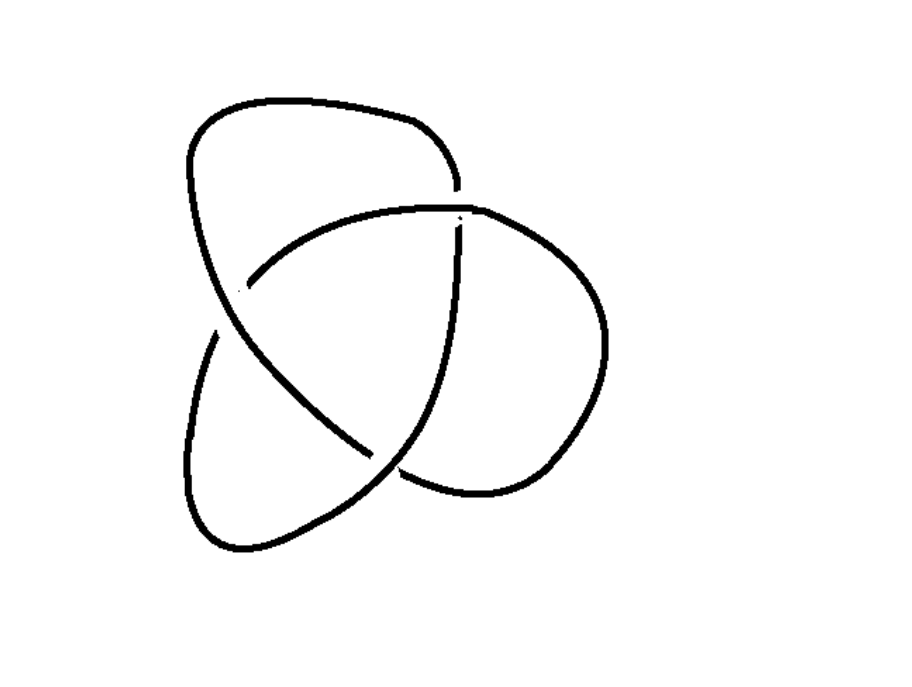
\includegraphics[width=0.46\linewidth]{fig01.png}
  \caption{嵌入于 $\R^3$ 中的纽结。\quad（原文 Figure~1，第 1 页）}
  \label{fig:1}
\end{figure}

% [Tutor Note: 这里是全文的逻辑枢纽，也是第一次出现“拓扑不变量落在 Z-torsor 中”的
%  含糊点。作者脚注只说是 Chern-Simons 标架反常，实际上：4 维规范场论中
%  n = (1/8π²)∫Tr F∧F 只在流形闭且丛平凡化时才是整数；当边界上丛被固定但未平凡化时，
%  n 只有在选定 W 与 K 的标架后才成为整数。第二讲式 (2.1) 之后会正面处理此事。
%  阅读时不要把“a_n 是整数”当作定义的一部分。]

为了得到 Khovanov 同调，上述情形应当被“范畴化”（categorified）：
也就是说，我们要对每个 $n$ 定义一个向量空间复形，使其欧拉示性数为 $a_n$。
据我所知，能够自然地范畴化“方程解的计数”的普遍情形只有一种：
我们所计数的方程恰好描述某个 Morse 函数 $h$ 的临界点。我们将处在这一框架之中。
我们的方程是偏微分方程（PDE），因此 $h$ 将是无穷维函数空间（即 PDE 中出现的函数构成的空间）
上的 Morse 函数；范畴化将涉及该函数空间的“中间维数”上同调理论，类似于 Floer 理论。
先把这一点搁置一旁，假定我们只是想描述未范畴化的理论，即 Jones 多项式。

% [Tutor Note: “中间维数上同调”指 Floer 理论中的 Maslov 指标/相对维数：
%  无穷维函数空间上 Morse 函数的临界点指标是无穷大，通常的做法是取
%  其与某个固定临界点的“相对指标”（Fredholm 指标），由此得到有限维的分次。
%  作者后文（式 1.14 前后）会把它落实为泛函 Γ(A,φ) 的临界点问题。]

如果直接写下来而不解释其来源，我声称应当计数以定义 Jones 多项式、
并最终定义 Khovanov 同调的那些方程，可能会显得随意（ad hoc）。
我本可以在今天开场时先讲解物理设定，但这对某些听众未必有帮助。
于是我决定改用另一条进路：通过与该领域已有的数学进路——即辛 Khovanov 同调
\cite{SS,Manolescu,AS}——作比较，来为这些方程提供动机。

% [Tutor Note: 这一段是 Witten 讲座的一贯风格：先声明“方程可能显得随意”，
%  再用数学上已知的构造反推。读者若只想要方程，可直接跳到式 (1.10)。]

回溯到 Vaughn Jones 的最初工作 \cite{Jones}，Jones 多项式的大多数进路都是
用纽结的某种“展示”（presentation）来定义不变量，例如投影到平面上——
就像画图~\ref{fig:1} 时所用的投影那样。人们先定义某个在给定展示下
显然良定义且可显式计算的东西；它是否与纽结的展示无关并不显然，但结果确实无关。
奥妙就在这一步。而奥妙总是有的。

% [Tutor Note: 原文写作 “Vaughn Jones”，标准拼写为 Vaughan Jones，属原文笔误，
%  此处照录。又，“presentation”在此译作“展示”（纽结的投影图/组合表示），
%  与群论中的“表现”同词不同义，注意区分。]

基于数 PDE 的解的进路，其优缺点恰好相反：拓扑不变性在原则上是显然的
（假定关于椭圆型 PDE 的某些一般性结论成立，并且紧致性得到控制），
但如何计算却不清楚。理想的情形是：既具有显然的三维（在范畴化情形为四维）对称性，
又有计算方法。这该如何实现？

% [Tutor Note: “topological invariance is potentially manifest” 一句是这一进路的
%  全部要点：只要方程是椭圆型的、解空间紧致、计数按代数方式定义，则解空间在
%  流形的微分同胚下不变，无需像 Jones 多项式那样去验证投影图的 Reidemeister 移动。
%  代价是紧致性极难证明——这正是第二讲末尾“compactness not yet proved”所指。]

我将说明如何从对辛 Khovanov 同调的了解出发，猜出正确的方程。
但要做到这一点，我们需要知道“实际去数一个方程的解”可能采取何种策略。
因此我先解释：假如已经知道要分析哪些方程，我们会怎么做——这会有助于我们猜出方程。

有一个标准的策略，适用于当前问题，可以在适当条件下尝试数出 PDE 的解。
其原始版本是关于三维流形 Floer 同调的 Atiyah--Floer 猜想 \cite{Atiyah}。
把他们的做法搬到当前问题上，想法是：把纽结沿某个方向（比如 $u$ 方向）拉长，
如图~\ref{fig:2} 所示；然后我们希望，除两端附近之外，解与 $u$ 无关。
这并非自动成立；在 \cite{GW} 中（该文对本问题采用了这一策略），
必须对方程组作微扰、使其变为更一般的方程组，才能达到这种情形。

\begin{figure}[H]
  \centering
  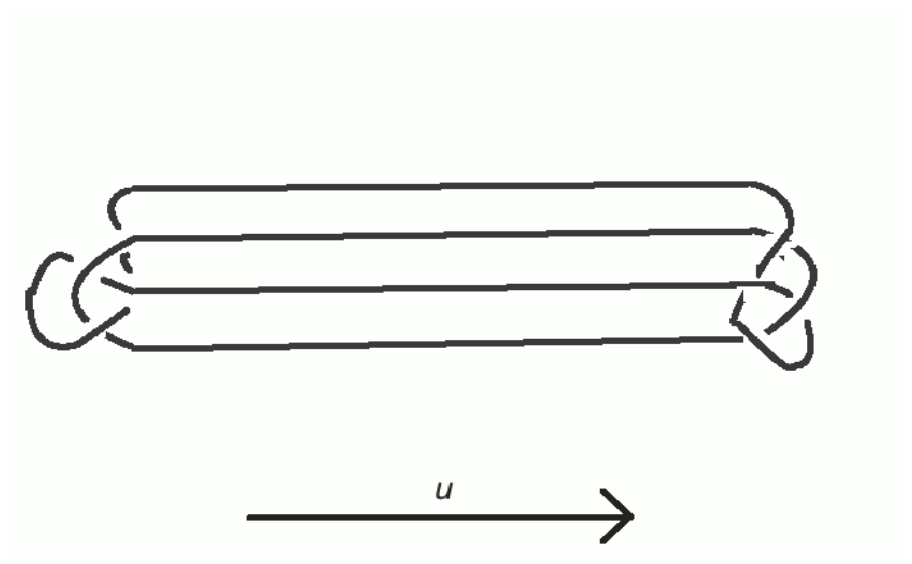
\includegraphics[width=0.46\linewidth]{fig02.png}
  \caption{嵌入于 $\R^3$ 中、并沿一个方向被拉长的纽结。\quad（原文 Figure~2，第 3 页）}
  \label{fig:2}
\end{figure}

% [Tutor Note: 这是全篇最容易被误读为“显然”的一步。拉长纽结后解趋于
%  u-无关，本质上是椭圆型方程在长柱面上的“指数衰减/收敛到平移不变解”，
%  需要一致的椭圆估计与紧致性；作者用“make a perturbation”一笔带过，
%  是因为在 [11]（Gaiotto–Witten）中已详细处理。若要做严格数学，
%  应查 [11] 与 [21]（Mazzeo–Witten）中关于退化椭圆算子的写法。]

既然如此，我们定义 $u$-无关解的模空间 $\sM$。可以把它们想象为：
在沿 $u$ 方向延伸的无穷多条平行股线存在时的解，如图~\ref{fig:3} 所示。

\begin{figure}[H]
  \centering
  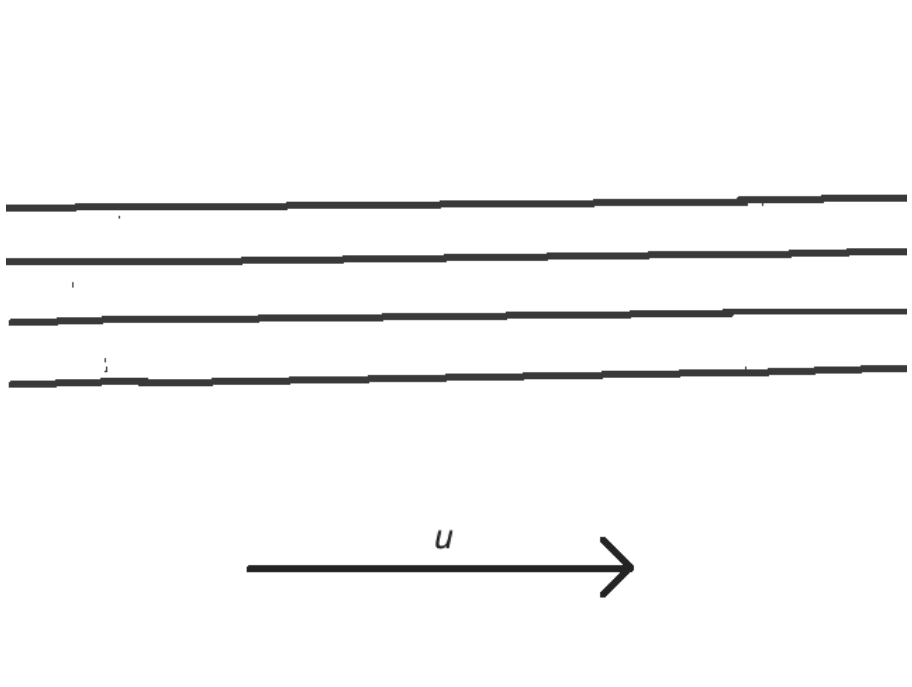
\includegraphics[width=0.46\linewidth]{fig03.png}
  \caption{以 $u$ 为参数的无穷多条平行股线，$-\infty\le u\le\infty$。
          \quad（原文 Figure~3，第 3 页）}
  \label{fig:3}
\end{figure}

现在如图~\ref{fig:4} 所示，考虑存在半无限股线时的解，这些股线延伸到
$u=+\infty$ 或 $u=-\infty$，但不会同时延伸到两端。
设 $\sL_\ell$ 与 $\sL_r$ 是这类解的模空间。于是 $\sL_\ell$ 中的点代表
一种半无限情形下的解，其中股线在左侧终止（如图~\ref{fig:4} 所画）；
类似地，$\sL_r$ 参数化股线在右侧终止的半无限情形下的解。
我们假定：这种半无限情形下的解在 $u\to+\infty$ 或 $u\to-\infty$ 时分别与 $u$ 无关。
若果真如此，则 $\sL_\ell$ 与 $\sL_r$ 都带有到 $\sM$ 的自然映射。
为术语简便起见，我们假定这些映射是嵌入；这等价于假定：
图~\ref{fig:2} 中内部的每个解至多只有一种方式向左或向右延拓。
这一假定并非必要，但能使解释简化。

\begin{figure}[H]
  \centering
  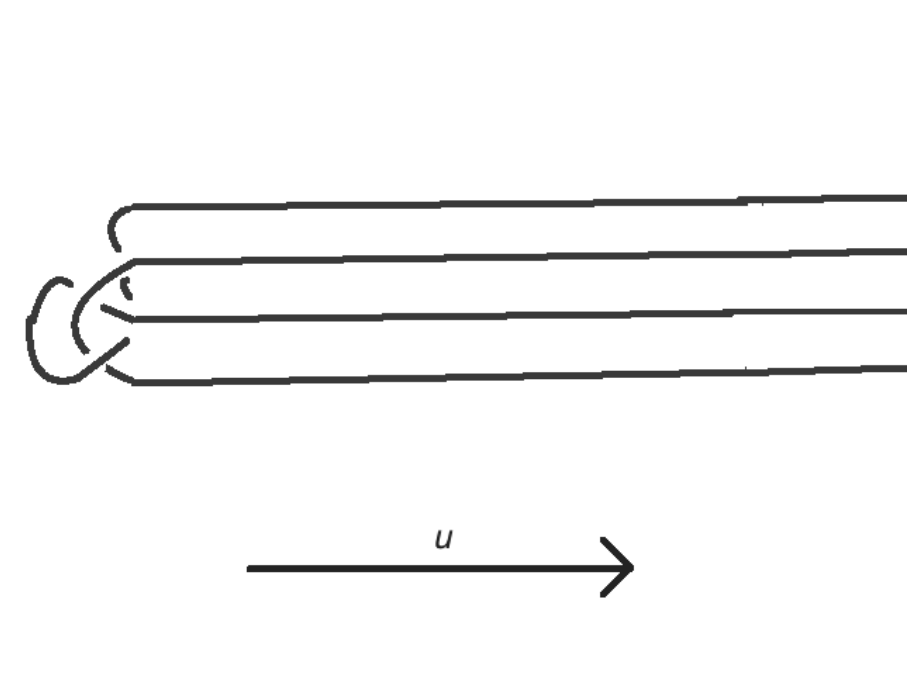
\includegraphics[width=0.46\linewidth]{fig04.png}
  \caption{延伸到 $u=+\infty$ 的半无限股线。\quad（原文 Figure~4，第 3 页）}
  \label{fig:4}
\end{figure}

像图~\ref{fig:2} 那样的整体纽结的解，可以理解为“在中间、同时向两端延拓”的解。
于是整体解就是 $\sL_\ell$ 与 $\sL_r$ 的交点。
作为 Jones 多项式系数的整数 $a_n$，应当就是 $\sL_\ell$ 与 $\sL_r$ 的代数相交数：
\begin{equation}\stepcounter{equation}
  a_n=\sL_\ell\cap\sL_r .
  \tag{1.2}\label{eq:1.2}
\end{equation}
（更确切地说，$a_n$ 是只计入满足 $P=n$ 的交点后所得的相交数。）

% [Tutor Note: 式 (1.2) 的写法在记号上偷了懒：左边是数、右边是集合的“交”。
%  严格说法是：在 $\sM$ 中 $\sL_\ell$ 与 $\sL_r$ 横截相交，交点为有限集，
%  每个交点带符号（由二者的定向决定），$a_n$ 是其代数和，并只取 P=n 的那部分。
%  这种“交点数 = 系数”的写法是 Floer 理论的标准简写，后文 (1.16)、(2.2) 同理。]

在这种“相交”的语言里，若 $\sM$ 自然地是辛流形、且 $\sL_\ell$ 与 $\sL_r$
是拉格朗日子流形，范畴化就有可能实现。此时 $\sM$ 的 Floer 上同调——
即 A-模型或 Fukaya 范畴——给出了范畴化的框架。
从今天讲座的观点看，这一切之所以会发生，是因为：甚至在我们把纽结拉长、
化归为 $\sM$ 中的交点之前，我们所计数的方程本身就已经是某个 Morse 泛函 $h$
的临界点方程。

% [Tutor Note: 这里的逻辑链要看清：(i) 方程 = 泛函临界点方程 ⇒ Morse/Floer 范畴化；
%  (ii) 拉长后解空间 = 两个拉格朗日子流形的交点 ⇒ 可用 Fukaya 范畴。
%  两条路给出同一个范畴化，这正是作者说“even before we stretched”之意。
%  容易混淆的是：辛 Khovanov 同调里 M 是有限维超 Kähler 流形，
%  而这里的 Morse 泛函是无穷维的；二者通过“降维”对应，见下文。]

\subsection{Hecke 修正、辛 Khovanov 同调与模空间}

在“辛 Khovanov 同调”中，人们针对 Khovanov 同调（至少是单分次版本）
发展出了这样一套故事，所用的 $\sM$ 非常具体。\cite{Kamnitzer} 提出了
关于这个 $\sM$ 的一种描述（并在 \cite{CK} 中以镜像版本加以利用），
它也为我的工作提供了重要线索；该描述如下：$\sM$ 可以理解为 Hecke 修正的空间。
让我解释这个概念。设 $C$ 是 Riemann 曲面，$E\to C$ 是 $C$ 上的全纯 $\Gc$-丛，
其中 $\Gc$ 是某个复 Lie 群。$E$ 在点 $p\in C$ 处的 Hecke 修正是
一个全纯 $\Gc$-丛 $E'\to C$，连同它在 $p$ 之外与 $E$ 的同构：
\begin{equation}\stepcounter{equation}
  \varphi:\; E'\big|_{C\setminus p}\;\cong\; E\big|_{C\setminus p}.
  \tag{1.3}\label{eq:1.3}
\end{equation}

% [Tutor Note: 原文排版把式 (1.3) 的限制符号拆成两行（C\p 与 C\p 分列），
%  这是 dvips 分式排版的产物，不是笔误；此处照原意排版。
%  Hecke 修正的要点是：在 p 点“允许一个极点/零点”，而在别处保持同构。
%  这一概念在几何 Langlands 中是基本对象；参见 [15]（Kapustin–Witten）§3。]

例如，若 $\Gc=\CC^{*}$，则可以把 $E$ 看作全纯线丛 $\sL\to C$。
在 $p$ 之外与 $\sL$ 同构的全纯丛 $\sL'$ 必形如
\begin{equation}\stepcounter{equation}
  \sL'=\sL(np)=\sL\otimes\sO(p)^{n}
  \tag{1.4}\label{eq:1.4}
\end{equation}
其中 $n$ 为某整数。这里 $n$ 可以看作 $\CC^{*}$ 的 Langlands--GNO 对偶群的权；
后者是另一份 $\CC^{*}$。

% [Tutor Note: 原文 “the we can think of E” 应为 “then we can think of E”，
%  属笔误，照录。
%  另注：\sL(np) 表示把 \sL 在 p 处的局部生成元乘以 z^{-n}，
%  即把“零点/极点的阶”改变 n；不同作者对 n 的符号约定相反，
%  本文取 E'=E(np) 为“增加 n 阶零点”，读 (1.8) 时须与这里一致。]

我之所以写 $\Gc$、明确标出这是群的复形式，是因为做规范场论时，
规范群将取紧实形式，我把它简记为 $G$。一般地，对任意 $G$，
都有相应的 Langlands--GNO 对偶群 $\Gv$，其复化为 $\Gv_{\CC}$，
使得全纯 $\Gc$-丛在点 $p\in C$ 处的 Hecke 修正构成以支配权
（等价地，以 $\Gv_{\CC}$ 的有限维表示）分类的族。

% [Tutor Note: “families classified by dominant weights” 一句是本节的数学核心，
%  但作者没有给出证明。其根据是 Beilinson–Drinfeld / 仿射 Grassmann 流形的
%  几何 Satake 等价：p 点处允许的修正由 G^∨ 的支配权标号，
%  每个支配权对应一族（一个“ Schubert 胞腔”）。可查 [12]（Kamnitzer）
%  与 [15] 的相关章节。文中 G^∨_C 的角标 C 在 dvips 输出里被排到下一行，
%  这是排版问题，不是“复化”之外的另一个群。]

例如，若 $\Gc=GL(2,\CC)$，则可以把 $\Gc$-丛 $E\to C$ 看作秩 2 复向量丛
$E\to C$。Langlands--GNO 对偶群 $\Gv_{\CC}$ 仍是 $GL(2,\CC)$；
与 $\Gv_{\CC}$ 的二维表示对偶的 Hecke 修正如下：在 $p\in C$ 的某邻域内
取局部分解 $E\cong\sO\oplus\sO$，则 $E'\cong\sO(p)\oplus\sO$。
与交换情形不同之处在于：$p$ 处这种类型的 Hecke 修正不止一个，而是一整族，
它来自“选取 $E$ 的一个将被 $\sO(p)$ 替换的子丛 $\sO$”的自由度。

% [Tutor Note: 原文此处写作 “The Langlanda-GNO dual group”，
%  显系 “Langlands-GNO” 之误，属原文笔误，照录并标注。
%  又：这一步的“族”参数空间正是 \CC\PP^1 —— 选一个子线丛 O ⊂ O⊕O
%  等价于选一个点 [1:λ] ∈ CP^1。下一段会用到这一点。]

由于这种依赖性，$p$ 处这一类型的 Hecke 修正构成一个族，以 $\CP^1$ 为参数。
今设有 $2n$ 个点位于 $\CC\cong\R^2$ 上，我们要在平凡秩 2 复向量丛 $E\to\CC$
（图~\ref{fig:5}）的这些点上作这种类型的 Hecke 修正。所有这些 Hecke 修正构成的空间
将是 $(\CP^1)^{2n}$ 的一份拷贝，每个点处一份 $\CP^1$。
然而，其中有一个自然子簇 $\sM\subset(\CP^1)^{2n}$，定义如下：
在 $\CC$ 上添上无穷远点 $\infty$ 而紧化为 $\CP^1$，于是我们是在对
$\CP^1$ 上的平凡丛 $E=\sO\oplus\sO$ 作 Hecke 修正。
$(\CP^1)^{2n}$ 中的一点给出在 $p_1,p_2,\dots,p_{2n}$ 处作 Hecke 修正、
得到新丛 $E'$ 的一种方式。空间 $\sM$ 由要求 $E'\otimes\sO(-n\infty)$ 平凡来定义。
（若我们在 $PGL(2,\CC)$ 而非 $GL(2,\CC)$ 中工作，那就只需说 $E'$ 应当平凡。）

\begin{figure}[H]
  \centering
  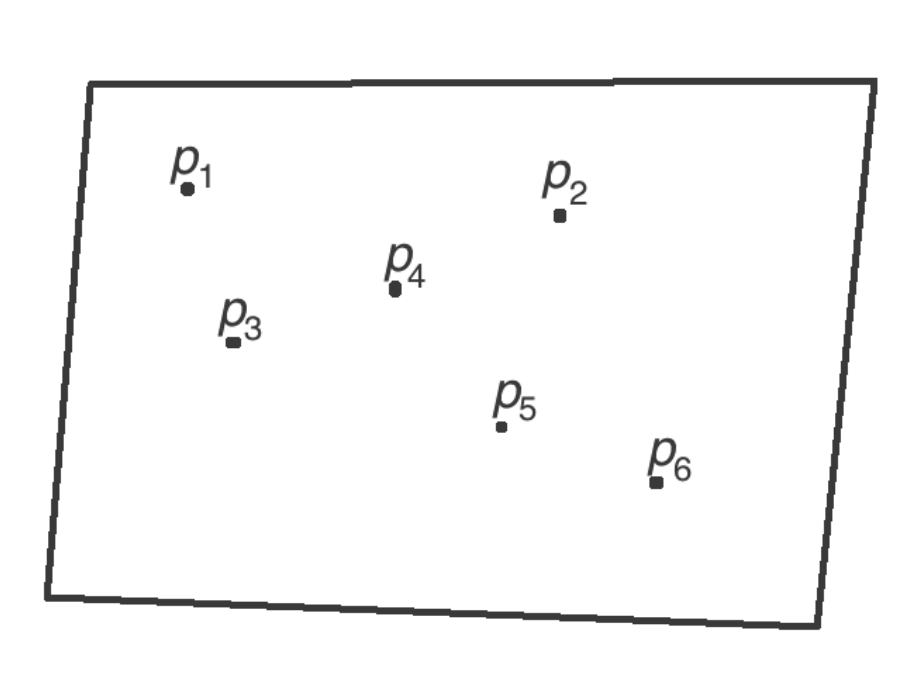
\includegraphics[width=0.46\linewidth]{fig05.png}
  \caption{点 $p_i\in\R^2$ 的构型，我们要在这些点处作 Hecke 修正。
          \quad（原文 Figure~5，第 5 页）}
  \label{fig:5}
\end{figure}

% [Tutor Note: 这里的 \sM ⊂ (CP^1)^{2n} 是“仿射 Grassmann 流形的多重点版本”，
%  也就是 Kronheimer 的引力瞬子模空间的另一种描述。条件 E'⊗O(−n∞) 平凡，
%  是在说“整体上丛的度数为零”，即修正前后总 Chern 类不变；
%  注意 \sM 的维数是复 2n−2（而不是 2n），因为该条件切掉两个复维度。
%  作者把 GL 与 PGL 的差别放在括号里，是因为：在 GL 情形需要处理行列式线丛，
%  在 PGL 情形 CP^1 上的丛平凡性本身就已足够。此点在后文 B 场/IIA 的物理实现中
%  对应“整体 U(1) 因子的处理”，读附录时宜回来对照。]

辛 Khovanov 同调是通过考虑这样一个空间中的拉格朗日子流形之交来构造的：
该空间是“从平凡丛到自身的多重 Hecke 修正”构成的 $\sM$。
我们要用规范场论 PDE 重新解释它。

我与 Kapustin 关于规范场论与几何 Langlands 的工作 \cite{KW} 中，
一个重要的事实是：$\sM$ 可以实现为某个 PDE 方程组的解的模空间。
然而，尽管 $\sM$ 是用 2 维流形 $\R^2\cong\CC$ 上的丛来定义的，
那些 PDE 却是在 3 维空间——即 $\R^3$——上的。
因此，本讲余下的内容都会处在一个比预期多一维的维度里。
为描述 Jones 多项式（3 维空间中纽结的不变量），我们要数 4 维中某些 PDE 的解；
而范畴化的版本——Khovanov 同调——将涉及 5 维中的 PDE。

% [Tutor Note: 全篇最容易让人“掉维度”的一段。记法上：
%  模空间 \sM 是 2 维 C 上的对象，但其定义方程（Bogomolny）活在 3 维；
%  把 3 维解“升维”到 4 维的是 KW 方程；再升到 5 维的是 HW 方程（梯度流）。
%  每升一维，范畴化/分次的含义就多一层。读第二讲时请牢记这三层结构。]

% ===================== 第一讲（续） =====================

\subsection{Bogomolny 方程及其奇异解}

我们所需的三维 PDE 就是所谓的 \textbf{Bogomolny 方程}。它们是定义在
定向三维 Riemann 流形 $W_3$ 上、关于一对场 $A,\phi$ 的方程：
$A$ 是 $G$-丛 $E\to W_3$ 上的联络，$\phi$ 是 $\ad(E)\to W_3$ 的截面
（即一个取伴随值的 $0$-形式）。若 $F=\mathrm{d}A+A\wedge A$ 是 $A$ 的曲率，
则 Bogomolny 方程为
\begin{equation}\stepcounter{equation}
  F=\star\,\dA\phi .
  \tag{1.5}\label{eq:1.5}
\end{equation}
（这里 $\star$ 是 Hodge 星，$\dA$ 是外微分的规范协变推广。）

% [Tutor Note: 符号约定务必留心。本文采用数学家的约定：F = dA + A∧A，
%  协变导数 d_A = d + [A,·]；物理文献常写成 F = dA − iA∧A、D = d − iA。
%  两者相差 A → −iA 的替换，Bogomolny 方程的形状 F = ⋆d_Aφ 不变。
%  另外 ⋆d_Aφ 中 ⋆ 作用在 2-形式上——验证时请记住 3 维中 ⋆: Ω² → Ω¹。
%  与第二讲的 KW 方程 F − φ∧φ = ⋆d_Aφ 对照可见：丢掉 φ∧φ 项、（把 φ 视作 0-形式）即回到此处。
%  记号 (A,φ) 中 φ 在 3 维是 0-形式，在 4 维是 1-形式，切勿混淆。]

Bogomolny 方程有许多非凡的性质，我们只关注其中一个方面。
考虑 $W_3=\R\times C$ 上的 Bogomolny 方程，其中 $C$ 是 Riemann 曲面。
$G$-丛 $E\to C$ 上的任何联络 $A$ 都在 $E$（更确切地说，在其复化）上决定一个全纯结构：
只需写 $\dA=\overline{\partial}_A+\partial_A$，并用 $\overline{\partial}_A$ 定义复结构。
（在复维数 1 的情形，$\overline{\partial}$ 算子无需满足任何可积性条件。）
因此，对任意 $y\in\R$，把 $E\to\R\times C$ 限制到 $E\to\{y\}\times C$，
就得到全纯丛 $E_y\to C$。然而，若 Bogomolny 方程被满足，$E_y$ 便典范地与 $y$ 无关。
事实上，Bogomolny 方程的一个推论是：$\overline{\partial}_A$ 在共轭意义下与 $y$ 无关。
若用 $y$ 参数化 $\R$，则 Bogomolny 方程蕴含
\begin{equation}\stepcounter{equation}
  \left[\frac{D}{Dy}-\mathrm{i}\phi,\;\overline{\partial}_A\right]=0 .
  \tag{1.6}\label{eq:1.6}
\end{equation}
于是 $\overline{\partial}_A$ 在自然的共轭意义下与 $y$ 无关。

% [Tutor Note: 此处推导极易出现符号错误。由 Bogomolny 方程 F = ⋆d_Aφ 的
%  分量形式，在 W₃ = R×C 上取 y 方向分量可推出 D_y φ = ⋆F 的相应分量，
%  再与 ∂̄_A 对易即得 (1.6)。注意：原文写 D/Dy − iφ，若改用物理约定
%  D = ∂ − iA 则同一方程写成 [D_y − iφ, ∂̄_A] = 0；若把 φ 换成 −φ，
%  则 i 的符号随之翻转。文中 “up to conjugation” 的共轭由 (1.6) 中的
%  对易子给出：∂̄_A 与 e^{...} 的共轭相等，而非严格相等。
%  更细的推导可查 [15] §3.1（Kapustin–Witten 对偶的方程部分）。]

Bogomolny 方程允许在孤立点处带奇点的解。为理解基本图像，我们取三维流形为
$\R^3$、规范群为 $U(1)$。固定整数 $n$，可以观察到 Bogomolny 方程对任意
$x_0\in\R^3$ 都有精确解
\begin{equation}\stepcounter{equation}
  \phi=\frac{n}{2|\vx-\vx_0|},\qquad F=\star\,\mathrm{d}\phi .
  \tag{1.7}\label{eq:1.7}
\end{equation}
我只定义了 $F$，而没有定义以 $F$ 为曲率的联络 $A$，也没有定义 $A$ 所联络的线丛 $\sL$。
这样的 $\sL$ 与 $A$ 存在（且本质上唯一）当且仅当 $n\in\ZZ$。

% [Tutor Note: 这正是 Dirac 磁单极（及其“Dirac 弦”）。n ∈ Z 的原因是：
%  在去掉奇点后的 R³\{pt} 上，F 的积分给出第一 Chern 数，
%  而 U(1) 丛的过渡函数必须单值，故 (1/2π)∫F ∈ Z。
%  这里 φ = n/(2r) 是“极点解”/Nahm 极点的雏形——第二讲中把它沿一条直线延拓，
%  就得到 Nahm 极点边界条件。注意本文的 1/(2r) 归一化使 ∫_{S²} ⋆dφ = 2πn。]

对 $G=U(1)$，由于 Bogomolny 方程是线性的，它可以有唯一解：
在指定的点 $p_i\in\R^3$ 处具有由指定整数 $n_1,n_2,\dots$ 标记的这类奇点（图~\ref{fig:6}）。
我们简单地取 $\phi=\sum_i\frac{n_i}{2|\vx-\vx_i|}$、$F=\star\,\mathrm{d}\phi$。
我们假定 $\sum_i n_i=0$，这保证 $\phi$ 与联络 $A$ 在无穷远处比 $1/|\vx|$ 更快地趋于零。

\begin{figure}[H]
  \centering
  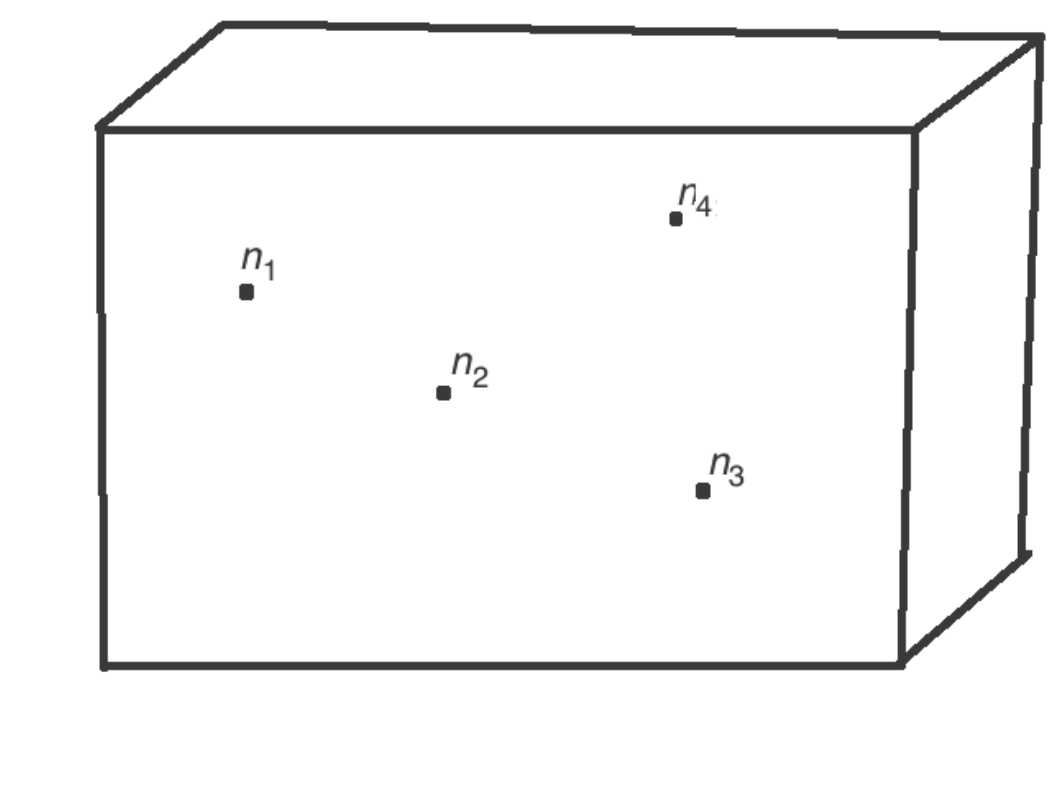
\includegraphics[width=0.46\linewidth]{fig06.png}
  \caption{点 $y_i\times p_i\in\R^3$，以群 $U(1)$ 的权 $n_i$ 标记。
          \quad（原文 Figure~6，第 7 页）}
  \label{fig:6}
\end{figure}

现在取分解 $\R^3=\R\times\R^2$，并把 $\R^2$ 认同为 $\CC$。设奇点位于
$y_i\times p_i$，其中 $y_i\in\R$、$p_i\in\CC$。对每个
$y\notin\{y_1,\dots,y_n\}$，上述 Bogomolny 方程的解决定一个全纯线丛
$\sL_y\to\CC$；加上无穷远点后，它自然延拓为 $\sL_y\to\CP^1$。
（这里用到了 $A$ 在无穷远处比 $1/|\vx|$ 更快趋于零这一事实。）
只要 $y$ 不等于某个 $y_i$，$\sL_y$ 在相差同构的意义下与 $y$ 无关；
但即便 $y$ 越过某个 $y_i$，$\sL_y$ 限制到 $\CP^1\setminus p_i$ 上仍是不变的。
在越过 $y=y_i$ 时，$\sL_y$ 经历一次 Hecke 修正
\begin{equation}\stepcounter{equation}
  \sL_y\;\to\;\sL_y\otimes\sO(p_i)^{n_i}.
  \tag{1.8}\label{eq:1.8}
\end{equation}
当 $y\to-\infty$ 与 $y\to+\infty$ 时，$\sL_y$ 都是平凡的
（同样是因为解在无穷远处比 $1/|\vx|$ 更快趋于零）。
于是该解描述了一串从平凡丛到自身的 Hecke 修正。

% [Tutor Note: 式 (1.8) 的指数 n_i 的符号与 (1.4) 的约定相同：正 n_i 表示在 p_i 处
%  增加 n_i 阶零点。若按相反约定（把 O(p_i)^{n_i} 理解为增加极点），
%  则整篇文章所有 Hecke 修正的指数都要统一变号，不可只改一处。
%  又：Σ n_i = 0 保证 y → ±∞ 时丛平凡、φ → 0；若 Σ n_i ≠ 0，
%  则解在无穷远处不趋于零，需另行处理（对应非平凡整体单极子荷）。
%  另：\sL 在此既指全纯线丛——请与后文 (p.15) 用 \sL 表示“线性化算子”区分，
%  原文二者同用 \mathcal{L}，极易混淆。]

对任意单 Lie 群 $G$，可以作类似的事情。（其基本想法由 't Hooft 在 1970 年代后期
引入 \cite{tHooft}，在量子规范场论的物理应用中十分重要。）
设 $T$ 是 $G$ 的极大环面、$\Lie$ 是其 Lie 代数。取同态
$\rho:\ug\to\Lie$。在相差一个 Weyl 变换的意义下，这样的 $\rho$ 等价于对偶群
$\Gv$ 的一个支配权，因此对应 $\Gv$ 的一个表示 $R^{\vee}$。
我们把这个已经用过的 $U(1)$ Bogomolny 方程奇异解 (1.7)
（更确切地说，是该解在 $n=1$ 时的特殊情形）简单地通过
\begin{equation}\stepcounter{equation}
  (A,\phi)\;\to\;\bigl(\rho(A),\rho(\phi)\bigr)
  \tag{1.9}\label{eq:1.9}
\end{equation}
变成一个 $G$ 的奇异解。然后我们在指定点 $y_i\times p_i\in\R^3$ 处，
寻找具有这类奇点的 $G$-Bogomolny 方程的解。

% [Tutor Note: (1.9) 是所谓“'t Hooft 嵌入”：把 U(1) 的磁单极解经 homomorphism
%  ρ: u(1) → t 嵌入非交换规范群，得到带非阿贝尔磁荷的奇异解。
%  这里 ρ 既作用于联络（沿 t 方向的分量），也作用于 Higgs 场 φ，
%  是把 u(1)-值对象变到 g-值对象的唯一自然方式。注意 (A,φ) → (ρ(A),ρ(φ))
%  并不是一般规范变换，而是“把解限制到子代数再嵌入”，不改变 F = ⋆d_Aφ 的形状。
%  与第二讲的 't Hooft 面算子（surface operator）直接相关。]

图像与之前相同，只是现在（图~\ref{fig:7}）点 $y_i\times p_i$ 不再由整数 $n_i$ 标记，
而是由同态 $\rho_i:\ug\to\Lie$ 标记，换言之，由对偶群 $\Gv$ 的表示 $R^{\vee}$ 标记。
此外，现在我们必须要求解在无穷远处比 $1/r$ 更快地趋于零
（对 $U(1)$，一旦令 $\sum_i n_i=0$，这一点自动成立）。
有了这个条件，这样的解就描述了一串在 $p_i$ 处、类型为 $\rho_i$ 的 Hecke 修正，
它们把 $\CP^1$ 上的平凡 $G$-丛 $E$ 映到自身。

\begin{figure}[H]
  \centering
  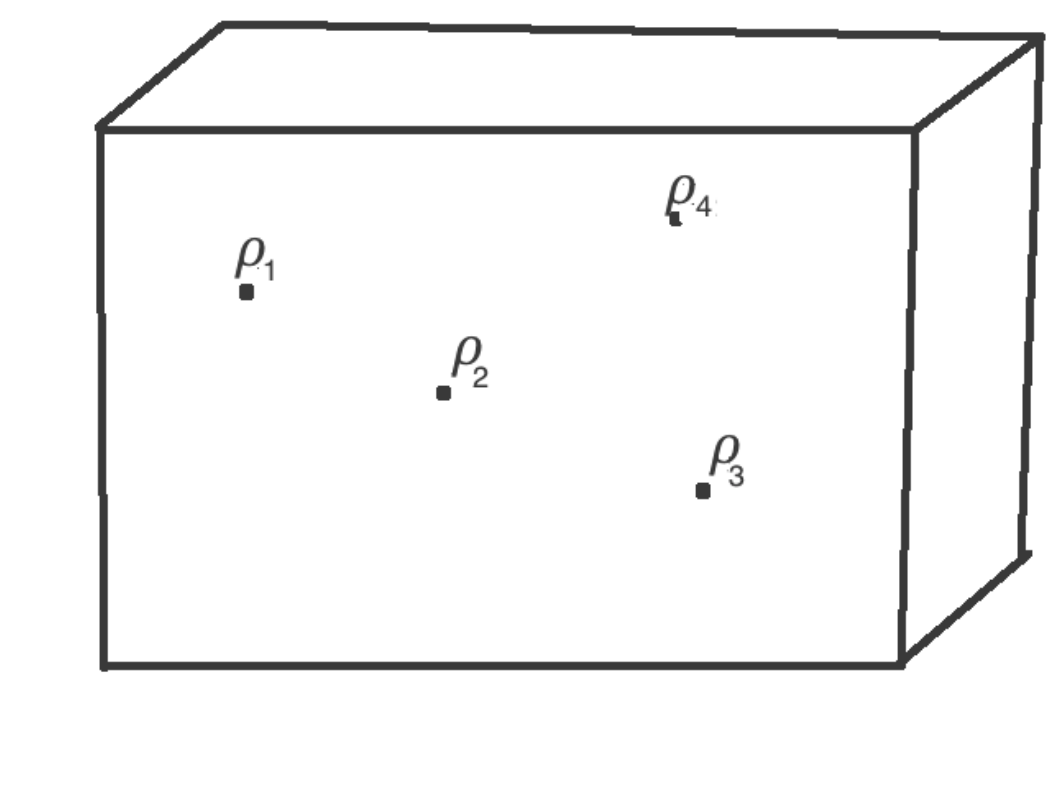
\includegraphics[width=0.46\linewidth]{fig07.png}
  \caption{$\R^3$ 中的点，由同态 $\rho_i:\ug\to\Lie$ 标记，
          或等价地由对偶群的表示标记。\quad（原文 Figure~7，第 8 页）}
  \label{fig:7}
\end{figure}

% [Tutor Note: “比 1/r 更快地趋于零”这一条件在非阿贝尔情形不是自动的：
%  Σ n_i = 0 只是保证 U(1) 部分没有单极荷；非阿贝尔情形还需所有
%  与 ρ 相关的整体荷为零，否则解在无穷远处有非平凡的渐近值。
%  这正是 [14]（'t Hooft）与 [15] 中所谓“在无穷远处趋于零”的精确含义，
%  作者在此一笔带过，读者切勿以为它与 U(1) 情形同样平凡。]

在 $\R^3$ 上、带上述奇点且在无穷远处比 $1/r$ 更快趋于零的 Bogomolny 方程
解的模空间 $\sM$，实际上是一个超 Kähler 流形，最初由 P. Kronheimer 在 1980 年代研究过。
若取分解 $\R^3=\R\times\R^2$，这就挑出了超 Kähler 流形上的一个复结构；
在该复结构下，$\sM$ 就是在指定点处、具有指定类型的全部 Hecke 修正的模空间
$\sM_{p_1,\rho_1;p_2,\rho_2;\dots}$，这些修正把 $\CP^1$ 上的平凡丛映到自身。

% [Tutor Note: Kronheimer 的构造（“引力瞬子”）给出的恰是 ALE/ALF 空间上的
%  单极子模空间，其超 Kähler 结构来自 hyper-Kähler quotient（ADHM 型构造）。
%  这里的要点是：\sM 上的三个复结构对应 R³ 中三个方向的选取；
%  取定 R³ = R×R² 的分解 = 取定其中一个复结构（即选定“哪个方向是 y”）。
%  第二讲将会看到，这个“选定复结构”的操作对应 KW 方程中把 φ 视为 1-形式
%  并取某个 t ∈ RP¹ 的自对偶/反自对偶分解。]

这一构造可以用来解释 Hecke 修正空间的许多性质，但今天我们要聚焦于它在纽结理论中的应用。
化归到 $\sM$ 应当来自沿某个方向拉长纽结；因此我们希望 $\sM$ 是某个方程的
$u$-无关解的模空间，如图~\ref{fig:3} 所提示。我们已经用 $\R^3$ 上某些 PDE 的解描述了 $\sM$，
所以现在必须把 $\sM$ 想成 $\R^4=\R^3\times\R$ 上 $u$-无关解的模空间，
其中第二个因子由 $u$ 参数化。

\subsection{四维 Kapustin--Witten 方程}

确实存在可用的自然四维 PDE。它们在几何 Langlands 的规范场论进路 \cite{KW} 中扮演角色，
有时被称为 \textbf{KW 方程}。它们是关于一对场 $A,\phi$ 的方程：
$A$ 是 $E\to Y_4$ 上的联络（$Y_4$ 是四维流形），$\phi$ 是 $Y_4$ 上取值于 $\ad(E)$ 的 1-形式：
\begin{equation}\stepcounter{equation}
  F-\phi\wedge\phi=\star\,\dA\phi,\qquad \dA\star\phi=0 .
  \tag{1.10}\label{eq:1.10}
\end{equation}
在特殊情形 $Y_4=W_3\times\R$、$A$ 是自 $W_3$ 的拉回、且 $\phi=\varphi\,\mathrm{d}u$
（其中 $\varphi$ 是 $\ad(E)$ 的截面、$u$ 参数化 $Y_4$ 中的第二个因子）下，
这些方程约化为 $W_3$ 上的 Bogomolny 方程：
\begin{equation}\stepcounter{equation}
  F=\star\,\dA\varphi .
  \tag{1.11}\label{eq:1.11}
\end{equation}

% [Tutor Note: (1.10) 是 Kapustin–Witten 方程的标准形式（见 [15] eq. (2.2) 附近）。
%  两个易错点：(i) 这里 φ 是 1-形式，φ∧φ 不恒为零，且取 Lie 代数对易子；
%  (ii) ⋆ 在 4 维中把 2-形式映到 2-形式，故 F − φ∧φ 与 d_Aφ 同为 2-形式。
%  约化到 (1.11) 时要小心：φ = φ du 时 φ∧φ = 0，而 ⋆d_Aφ 中的 ⋆
%  是 4 维 Hodge 星；它作用在 du 上产生 3 维 Hodge 星，这才是 (1.11) 的由来。
%  不同文献对 (1.10) 的符号约定（F ± φ∧φ）不一致，本文取“减号”，
%  与 [15] 一致；若换成加号，则 t ∈ RP¹ 的参数化中 t 与 t^{-1} 互换。]

因此，我们先前研究过的 Bogomolny 方程奇异解 (1.9) 可以被提升为 KW 方程的奇异解；
只是现在奇点是沿着一条直线、而不是在一个点上。当然，奇点仍然处在余维 3。
我们把这个解看作一个模型，它告诉我们：在更一般的情形下应当寻找何种余维 3 奇点。
若 $Y_4$ 是四维流形、$S\subset Y_4$ 是嵌入的一维流形，并以同态
$\rho:\ug\to\Lie$（或 $\Gv$ 的一个表示）标记，则可以寻找 KW 方程的解，
使其沿 $S$ 具有与所选 $\rho$ 相应的奇点（图~\ref{fig:8}）。

\begin{figure}[H]
  \centering
  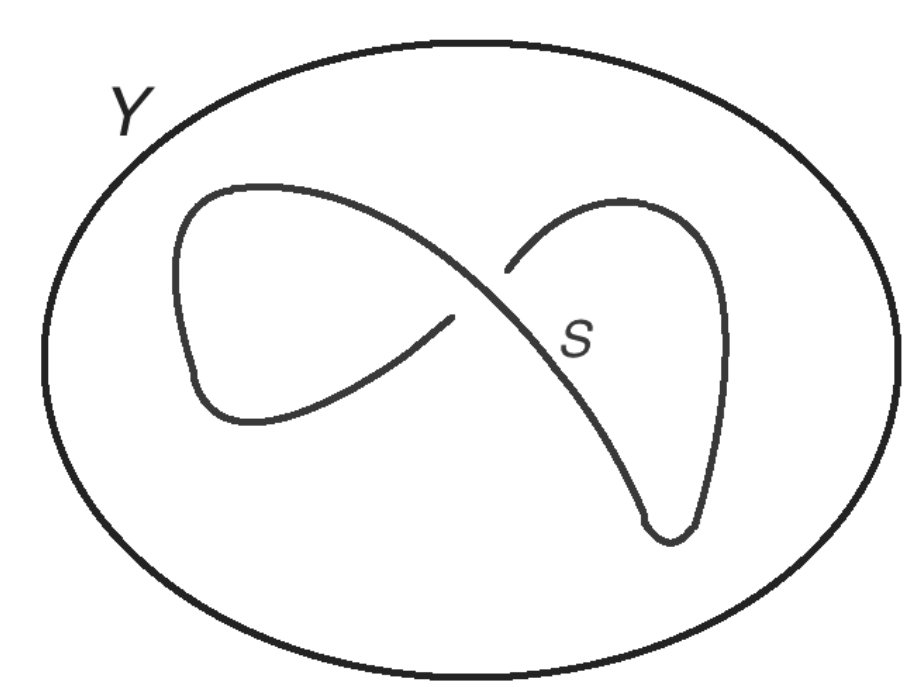
\includegraphics[width=0.46\linewidth]{fig08.png}
  \caption{四维流形 $Y$，其中嵌有一维流形 $S$；沿 $S$ 指定所要求的奇点。
          \quad（原文 Figure~8，第 9 页）}
  \label{fig:8}
\end{figure}

若我们特殊化到 $Y_4=\R^3\times\R$、$S=\cup_i S_i$、$S_i=p_i\times\R\subset\R^3\times\R$
（$p_i$ 是 $\R^3$ 中的点，$\R$ 由 $u$ 参数化）的情形，则 KW 方程的 $u$-无关解
正是 $\R^3$ 上 Bogomolny 方程带所选奇点的解。因此这些解由 $\sM$ 参数化；
而且确实可以证明，在无穷远处行为合理的条件下，这些就是该情形下 KW 方程的全部解。

% [Tutor Note: 最后一句“可以证明……全部解”是作者第二次略去细节之处：
%  需要用到关于解在 u → ±∞ 的指数衰减估计（沿 u 方向的 ODE 稳定性分析）。
%  若只关心 4 维方程本身，可把它当作工作假设；严格的证明思路见
%  [15] §3 与 [11]（Gaiotto–Witten）中关于拉伸极限的讨论。]

于是我们有了一个四维椭圆型 PDE，并且可以用有趣的方式指定它在嵌入圆周
$S\subset Y_4$ 上应当具有何种奇点。但这听起来像是给纽结理论准备的一个荒谬的框架，
因为一维流形在四维流形中根本不会“打结”！

\subsection{范畴化：Morse 同调与 HW 方程}

为了解决这一点，我们必须解释范畴化究竟涉及什么。让我们先用普通的方程
（而非偏微分方程）来练习。设 $N$ 是有限维紧定向流形，
$V\to N$ 是实向量丛，且 $\operatorname{rank}(V)=\dim N$。又设给定 $V$ 的一个截面 $s$。
通过带重数（特别是带符号）地计数 $s$ 的零点，我们可以定义一个整数。
这个整数就是 Euler 类 $\int_M\chi(V)$。

% [Tutor Note: 原文此处写作 \int_M χ(V)（CMMI 字体，确为希腊字母 χ），
%  这是作者本人的记号；Euler 类通常记作 e(V)，读者不必以为 χ(V) 是
%  Euler 示性数 χ(N)——它是 Euler 类配对流形的基本类所得的整数。
%  另：原文“This integer is the Euler class”严格说应是“Euler 类的积分”
%  （Euler 数是数、Euler 类是上同调类），此为口语化表述，照译。
%  还有一个隐含前提：s 横截于零截面，否则需按代数几何的方式计数。]

一般来说，据我所知，没有办法范畴化向量丛的 Euler 类。
然而，假定 $V=T^*N$ 且 $s=\mathrm{d}h$，其中 $h$ 是 Morse 函数。
那么 $s$ 的零点（即 $h$ 的临界点）有一种自然的“范畴化”，在 Morse 同调中加以描述。
人们定义一个复形 $\sV$，对 $h$ 的每个临界点 $p$ 取一个基向量 $\psi_p$。
该复形按 $\ZZ$ 分次：把 $p$ 的“指标”（Morse index）赋给 $\psi_p$；
它还有一个自然的微分，由计数不同临界点之间的梯度流线来定义。

具体地，微分定义为
\begin{equation}\stepcounter{equation}
  \mathrm{d}\psi_p=\sum_{q} n_{pq}\psi_q ,
  \tag{1.12}\label{eq:1.12}
\end{equation}
其中求和遍历所有 Morse 指标比 $p$ 大 1 的临界点 $q$，整数 $n_{pq}$ 由计数从 $p$ 到 $q$
的流（flow）来定义（图~\ref{fig:9}）。所谓“流”，是梯度流方程
\begin{equation}\stepcounter{equation}
  \frac{\mathrm{d}\vx}{\mathrm{d}t}=-\vnabla h
  \tag{1.13}\label{eq:1.13}
\end{equation}
的解。

\begin{figure}[H]
  \centering
  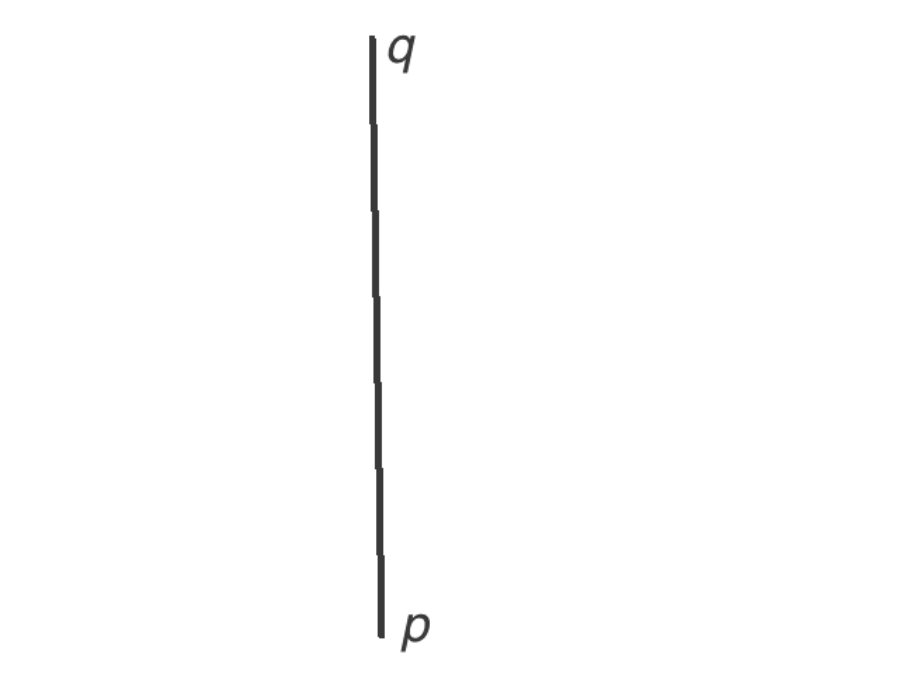
\includegraphics[width=0.38\linewidth]{fig09.png}
  \caption{从一个临界点流向另一个临界点。\quad（原文 Figure~9，第 10 页）}
  \label{fig:9}
\end{figure}

（为定义此方程，须在流形 $N$ 上取定一个 Riemann 度量。所得到的复形在拟同构意义下
与度量无关。我们考虑从 $p$（当 $t=-\infty$）出发、到 $q$（当 $t=+\infty$）终止的流。
这样的流构成经由时间平移相联系的单参数族，$n_{pq}$ 就是这种族的数目，按代数方式计数。）

% [Tutor Note: 这是全文对“范畴化”最具体的一段，务必读透：
%  (i) 复形 \sV 的基按临界点标号，微分次数 +1（指标增 1）；
%  (ii) 微分矩阵元 n_{pq} 是“模去时间平移的流线数”，即紧化模空间
%       的代数计数——若流线模空间是 0 维紧流形，则计数即带符号点数；
%       若维数 > 0，需要加微扰或取虚拟基本类；
%  (iii) 这里 Z 分次来自指标差，而“范畴化”的本质是把 Euler 类的计数
%       替换为链复形。原文“n_{pq} is the number of such families”一句
%       严格说是“计数模空间 \mathcal{M}(p,q)/R 的代数点数”，作者从简。
%  标准参考：Milnor, "Lectures on the h-cobordism theorem"；
%  Schwarz, "Morse Homology"；或 Witten 本人 1982 年关于 Morse 理论的论文。]

这就告诉我们，要想范畴化“数 KW 方程的解”这一问题，需要些什么。
我们必须能够把那些方程写成某个泛函 $\Gamma(A,\phi)$ 的临界点方程：
\begin{equation}\stepcounter{equation}
  \frac{\delta\Gamma}{\delta A}=\frac{\delta\Gamma}{\delta\phi}=0 .
  \tag{1.14}\label{eq:1.14}
\end{equation}
而相应的梯度流方程，将是 $X_5=\R\times Y_4$ 上的五维 PDE：
\begin{equation}\stepcounter{equation}
  \frac{\mathrm{d}A}{\mathrm{d}t}=-\frac{\delta\Gamma}{\delta A},
  \qquad
  \frac{\mathrm{d}\phi}{\mathrm{d}t}=-\frac{\delta\Gamma}{\delta\phi},
  \tag{1.15}\label{eq:1.15}
\end{equation}
它必须是椭圆型的，这样“数它的解”才有意义。

% [Tutor Note: 原文此处写作 “so that it will makes sense”，多一个 s，
%  属原文笔误，照录。
%  另外这里有一个概念上的要点：5 维方程是“梯度流”方程，因此其解空间的
%  Morse/Floer 理论给出 4 维方程解空间的范畴化——这正是“范畴化 = 升一维”
%  的技术含义。Gaiotto–Witten 的 HW 方程其实就是这些 5 维方程的具体形式。]

一般地，KW 方程在流形 $Y_4$ 上并不一定是某个泛函的临界点方程。
然而，若 $Y_4=W_3\times\R$（对某个 $W_3$），则确实如此。
若在嵌入的一维流形 $S\subset Y_4$ 上存在奇点，则还有一个进一步的条件：
在此情形下，KW 方程是某个泛函的临界点方程，当且仅当 $S$ 含于某个三维流形
$W_3\times p$ 之中，其中 $p$ 是 $\R$ 中的一点。
（关于“为什么”如此，请见附录。）

% [Tutor Note: 这是全篇最“物理”的一个断言，作者只给了判别准则而未证明。
%  其内容是：只有当奇点所在的一维流形完全落在某个“等 u”切片 W₃×p 内，
%  4 维方程才具有变分结构（存在 Γ）；否则（例如 S 斜着穿过 u 方向）
%  方程不来自泛函，只有 4 维方程而没有 5 维梯度流。
%  附录用 (0,2) 六维理论 + 拓扑全纯扭曲来解释“为什么”：
%  Q-不变性要求面算子沿 Σ×q′ 且 Σ ⊂ R⁴，这在约化后正是 S ⊂ W₃×p。
%  严格验证可对 (1.10) 逐分量检查：需要 φ 的 u-分量与 A_u 的某种组合消失。]

于是，为使范畴化成为可能，我们必须处在通向纽结理论的情形：
$S$ 是三维流形 $W_3$ 中的嵌入一维流形。一旦作出这一限制，
五维流方程就存在，而且确实是椭圆型的。（它们由 \cite{W5branes} 与 \cite{Haydys}
独立引入，有时被称为 \textbf{HW 方程}。）

% [Tutor Note: “HW”指 Haydys–Witten。作者在此把“范畴化所需的五大方程”
%  归功于 [3]（Witten, Fivebranes and knots）与 [19]（Haydys）两篇独立工作，
%  这是有争议的归属问题（另见 [18] 的讨论）；作者本人在脚注与正文中
%  并未声称原创性。读者若引用，宜同时列出二者。]

天真地说，这给出了对任意三维流形 $W_3$ 的“范畴化”纽结不变量；
但要论证这一主张，需要对所考虑方程的解有一定的紧致性性质。
我猜想，要正确证明这些紧致性性质，可能要求 $W_3$ 的 Ricci 张量非负——
这是一个非常强的限制条件。

% [Tutor Note: 这一段是作者少见的“坦白不确定性”之处，也是本领域至今
%  未解决的核心分析问题之一：在一般 W₃ 上，KW/HW 方程解空间的紧致性、
%  以及模空间的定向与虚拟基本类，都还没有完整的一般理论。
%  “Ricci 非负”的猜想对应的是：非负 Ricci 曲率下 Bochner 型公式可给出
%  解的一致估计。第二讲中 R_{ij} ≥ 0 的 Weitzenböck 公式正是同一想法的局部版本。
%  引用此文时请勿把“naively leads to”误读为定理。]

到目前为止我所描述的，应当对应（当 $W_3=\R^3$、$G=SO(3)$，且 $\rho$ 对应
$\Gv=SU(2)$ 的二维表示时）所谓的“单分次 Khovanov 同调”。
它之所以是单分次的，是因为我提到的唯一分次是与 Morse 指标相联系的分次，
换言之，与范畴化相联系的分次。在数学理论中，人们说：若把单分次的 Khovanov 同调
“去范畴化”并忘掉分次，它就变得平凡（即不能区分纽结）。
在我所描述的进路中，这一点成立，是因为在未范畴化的版本里，
嵌入的一维流形 $S$ 只是四维流形 $Y_4$ 中的一维流形
（它没有理由被嵌入三维流形 $W_3\times p$ 中），所以没有打结性可言。

% [Tutor Note: 这段解释了一个乍看奇怪的事实：单分次 Khovanov 同调
%  去范畴化后给出的是“平凡不变量”（即 Jones 多项式的某种退化），
%  而真正的 Jones 多项式需要 q-分次。作者用“1-流形在 4-维中不打结”
%  来解释为什么 4 维计数只给出单分次版本——这是本文的概念性洞见，
%  值得反复咀嚼：分次的信息 = 几何信息（能否把 S 限制到 3 维切片）。]

\subsection{q-分次与带边流形}

物理图像清楚地指出了 Khovanov 同调额外的“$q$”-分次应当从何而来。
它应当来自第二陈类（second Chern class）在四维流形 $Y_4$ 上的积分。
第二陈类就是我在本讲开头称作 $P$ 的那个不变量。
但出于拓扑上的原因，在我所描述的、沿嵌入一维流形 $S\subset Y_4$ 的余维 3 奇点存在时，
第二陈类无法定义。（由于奇点的存在，$Y_4$ 表现得像一个非紧四维流形，
其上不存在与 $G$-丛的第二陈类相对应的拓扑不变量。）
因此，到目前为止我所呈现的构造没有 $q$-分次。

% [Tutor Note: 这里的“拓扑原因”值得展开：若 S 是余维 3 的奇点轨迹，
%  在 S 的小管状邻域上丛的拓扑是非平凡的，Y₄ 的有效拓扑是“挖掉 S 后的开流形”，
%  而 H⁴ 不再有紧支类可供积分，故 ∫Tr F∧F 不是拓扑不变量（依赖于联络）。
%  第二讲的边界条件正是通过“在边界上固定丛但不平凡化”来恢复一个
%  良定义的（torsor 值的）第二陈数。这是全文第二讲的技术核心动机。]

物理图像告诉我们，要得到 $q$-分次该怎么做：$Y_4$ 应当是带边流形，
而纽结应放在它的边界里（图~\ref{fig:10}）。适当的边界条件将是第二讲的主题，
它使得第二陈类可以被定义。

\begin{figure}[H]
  \centering
  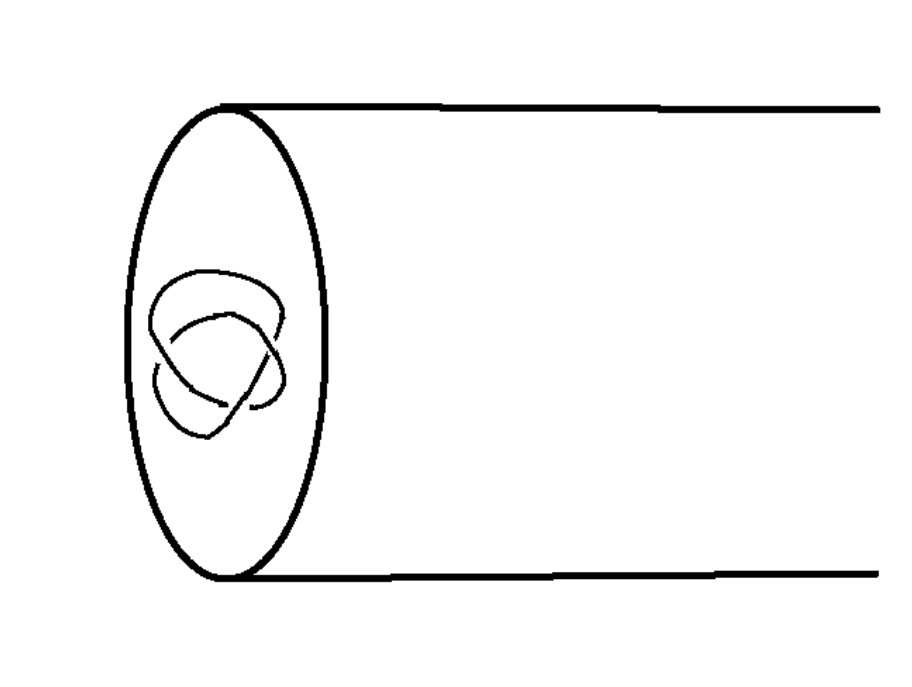
\includegraphics[width=0.46\linewidth]{fig10.png}
  \caption{带边的四维流形 $Y_4$，一个纽结被置于其边界中。
          \quad（原文 Figure~10，第 12 页）}
  \label{fig:10}
\end{figure}

在 \cite{GW} 中，Gaiotto 与我分析了这个问题（在未范畴化的情形，即我们数的是 4 维而非 5 维的解，
且只考虑最简单的 $G=SO(3)$ 情形），目的是不借助物理图像、直接证明 Jones 多项式为
\begin{equation}\stepcounter{equation}
  J(q)=\sum_{n}a_n q^{n},
  \tag{1.16}\label{eq:1.16}
\end{equation}
其中 $a_n$ 是具有第二陈类 $n$ 的解的数目。出发点是沿一个方向拉长纽结、
约化到低一维的方程，如图~\ref{fig:2} 所示。结果表明，低一维中满足边界条件的解
与大量有趣的数学物理相关，涉及可积系统、共形场论、几何 Langlands 等等。
由此浮现出来的是 Jones 多项式的“顶点模型”（vertex model）构造；
其浮现方式在某种程度上沿袭了 Bigelow \cite{Bigelow} 与 Lawrence \cite{Lawrence} 的工作。
我们的工作所增添的，是从一个具有显然三维对称性的出发点推导出顶点模型。
对于范畴化理论，其类似物预期（在某个版本中）会涉及带某个超势的 Fukaya–Seidel 范畴。
相关的模型——以及一个看似合理但行不通的变体——已在 \cite{GalakhovMoore} 中被探讨，
并在相当程度上被理解。

% [Tutor Note: 式 (1.16) 与 (1.1) 形式相同，但含义不同：(1.1) 是定义，
%  (1.16) 是 [11] 中试图证明的等式（用 4 维规范场论的解数重构 Jones 多项式）。
%  作者说“目的是直接证明”，但 [11] 实际得到的是“顶点模型”表示，
%  严格证明 Jones 多项式 = 解数这一等式仍未完成——这是本领域的公开问题。
%  读者引用时须区分“启发式推导”与“定理”。]

% ===================== 第二讲 =====================
\section{第二讲（Lecture Two）}
\label{sec:lecture-two}

\begin{keypoints}
  \item \textbf{物理图像}：要让第二陈类（即 $q$-分次）有意义，必须把纽结放到
        四维流形 $Y_4$ 的\textbf{边界}上，而不是让奇点沿内部的 1-流形分布。
        边界条件由“沿边界的奇异模型解 + 要求解渐近于它”来定义。
  \item \textbf{数学工具}：Nahm 极点边界条件、一致退化椭圆算子理论
        （Mazzeo–Witten）、Weitzenböck 公式族、仿射 Toda 方程、
        Fredholm 理论与指标、Bogomolny/Hitchin/Nahm 三类可积方程的“杂交”。
  \item \textbf{核心结论}：(i) Nahm 极点边界条件是椭圆边界条件，且其上同调
        给出空链环 Khovanov 同调秩为 1；(ii) 带纽结时，边界条件由
        以 $\Gv$ 的不可约表示 $R^{\vee}$ 标记的模型解定义，该模型解由
        仿射 Toda 方程给出；(iii) 相应的线性化算子核为零，从而边界条件
        在任意纽结 $K\subset W$ 存在时仍是椭圆/Fredholm 的。
\end{keypoints}

\subsection{边界条件与第二陈类}

在第一讲中我解释过：为在 Khovanov 同调中定义 $q$-分次，我们必须使
四维流形 $Y_4$ 上 KW 方程的解的第二陈类有意义——而且要在纽结存在的情形下。
如前所述，若纽结由余维 1 的嵌入子流形 $S\subset Y_4$ 表示，这是行不通的，
因为我们想沿 $S$ 假设的那种奇点不允许把第二陈类定义为一个拓扑不变量。
因此，我们改为把纽结嵌入 $Y_4$ 的边界中，如图~\ref{fig:10} 所示。
我们所用的边界条件描述起来颇为微妙，但它具有这样的性质：丛在边界上被固定，
因此第二陈类可以被定义。

% [Tutor Note: 注意“codimension 1 embedded submanifold S ⊂ Y₄”一句：
%  这是指把 3 维纽结放在 4 维流形的内部（余维 1），而非 4 维中的 1-流形。
%  原文此处用了“codimension 1”，与后文“codimension three singularity”
%  不是一回事：前者是 S 在 Y₄ 中的余维，后者是奇点在方程意义下的余维。
%  中文读者极易在此处混淆，特此标注。]

其实对任何带边的 $Y_4$ 都能得到 $q$-分次；但为了同时允许范畴化，
我们更具体地要求 $Y_4=W\times\R_+$，其中 $\R_+$ 是由 $y$ 参数化的半直线。
对于 Jones 多项式与 Khovanov 同调，我们进一步取 $W=\R^3$。
（更一般的 $W$ 当然也有趣，但人们对该期待什么所知甚少，参见 \cite{GPV}。）
于是如图~\ref{fig:10} 所勾画，$Y_4$ 就是 $\R^3\times\R_+$，纽结嵌入在其边界中。

% [Tutor Note: “W = R³”这一选择不是技术细节：它同时保证了 (i) 边界
%  W×{0} 上的 Nahm 极点边界条件可以取 Levi-Civita 联络（W 是平坦的），
%  (ii) 解在无穷远处可控，(iii) 与 Jones 多项式（R³ 中的纽结）对应。
%  对一般 W，边界条件需用 W 的度量/标架丛来写，见 [21]。[20]（Gukov–Putrov–Vafa）
%  讨论了更一般的 W 与 3-流形同调。]

% ===================== 第二讲（续一）：边界条件与 Nahm 极点 =====================

当 $y\to\infty$ 时，我们要求 $A,\phi\to 0$。当 $y\to 0$ 时，则有一个微妙的边界条件，
它是本理论的主要要点之一；描述它实际上是我今天的主要目标。
这个边界条件依赖于纽结 $K$，也依赖于 $K$（或链环 $L$ 的每个分支）由对偶群
$\Gv$（Langlands 或 GNO 对偶群）的一个表示 $R^{\vee}$ 所作的标记。
这是 $K$ 进入整个框架的唯一地方。

% [Tutor Note: “K 只从边界条件进入”是本文的结构性论断，值得强调：
%  4 维方程本身（KW 方程）与纽结无关；纽结的全部信息被编码在
%  “用哪个表示 R^∨ 标记、以及在边界上要求解渐近于哪个奇异模型解”之中。
%  这一点与 Chern–Simons 理论中“纽结 = Wilson 圈”的图景对偶：
%  在 CS 中纽结给出圈的可观测量的插入，在这里它变成边界条件的标记。
%  两种图景的对应正是 Gaiotto–Witten [11] 的核心内容。]

理想的边界条件是一个椭圆型边界条件，尽管它可能出人意料。
这里“椭圆型”的意思是：虽然定义看起来可能不寻常，但由此得到的性质
与更熟悉的椭圆型边界条件（如 Dirichlet 或 Neumann 条件）所得的性质类似。
例如，在紧四维流形上，KW 方程的线性化成为一个 Fredholm 算子，并具有离散谱。

在这个我将稍作详细描述的边界条件下，丛 $E$ 与联络 $A$ 限制到边界
$W\times\{y=0\}$ 上的取值是被指定好的。因此可以定义第二陈类
\begin{equation}\stepcounter{equation}
  n=\frac{1}{8\pi^{2}}\int_{W\times\R_+}\Tr\,F\wedge F .
  \tag{2.1}\label{eq:2.1}
\end{equation}
然而，由于丛在边界上被固定但并未被平凡化，这个不变量实际上取值于一个与
$W$ 和 $K$ 的标架（framings）相联系的 $\ZZ$-torsor。
“torsor”的意思是：$n$ 并非典范地就是一个整数；更确切地说，$n\bmod\ZZ$ 的值
只依赖于边界条件，而不依赖于满足该边界条件的具体规范场。
人们可以通过选取 $W$ 与 $K$ 的标架来“平凡化这个 torsor”，使 $n$ 成为整数。

% [Tutor Note: (2.1) 的归一化是关键：1/(8π²) 使瞬子数（instanton number）
%  在闭流形上为整数。这里 W×R₊ 是非紧的，但因边界上丛被固定，
%  积分仍收敛且由边界条件决定。若把 1/(8π²) 换成 1/(16π²) 或 1/(32π²)，
%  则 q 的指数整体平移/缩放，Jones 多项式的半整数指数（见第一讲脚注 2）
%  就不再与原文一致——这是校核时最容易出错的归一化常数之一。
%  另：torsor 一词在中文数学文献中常译作“主齐性空间”；
%  “framing”在此指流形切丛的平凡化（标架场），与纽结的“标架”是同一概念。]

为定义一个纽结多项式，人们（按标准方式带符号地）计数具有第二陈类 $n$ 的
KW 方程解的数目 $a_n$，然后定义
\begin{equation}\stepcounter{equation}
  J(q;K,R^{\vee})=\sum_{n\in\ZZ}a_n q^{n} .
  \tag{2.2}\label{eq:2.2}
\end{equation}
KW 方程解的紧致性（在适当的边界条件下尚未被证明）将意味着求和式中只有有限多项，
从而这是一个 Laurent 多项式。

% [Tutor Note: “尚未被证明”是作者 2016 年的判断；这句话是全文最重要的
%  开放性陈述之一。没有紧致性，a_n 可能为无穷大，(2.2) 只是形式级数。
%  注意即使紧致性成立，还需要“按代数方式计数”（即对模空间取虚拟基本类，
%  或对 Fredholm 算子取指标），才能得到与标架无关的整数 a_n。
%  作者在此用“in a standard way”一笔带过，实际是整套 Donaldson–Thomas/
%  Seiberg–Witten 式的技术。]

正如我在第一讲中解释过的，按此方式定义 Jones 多项式之后，
通向 Khovanov 同调的“范畴化”在原则上是很直接的。
它之所以出现，是因为 KW 方程可以在某种意义下被“提升”为五维中某些椭圆型微分方程，
而这些方程可以解释为梯度流方程。但今天我不再多谈这一点，
而是要描述四维（或五维）方程所需的那个边界条件。
这个边界条件属于可能有些陌生的类型，理解它对于在本课题上取得进展至关重要。

这些边界条件已在 \cite{MW} 中被研究，并在没有纽结的情形下被证明是椭圆型的。
关于带纽结情形的一篇文章正在撰写中 \cite{MWknots}，稍后我会就此略作介绍。
我将用四维方程的语言来展开讨论，因为如 \cite{MW} 所示，升到五维并没有太大变化。

% [Tutor Note: 作者把 5 维情形归约到 4 维的理由是：5 维方程 = 4 维方程的
%  梯度流，其“边界条件”在梯度流方向上的处理等价于对 4 维解空间的
%  Morse 理论要求；Mazzeo–Witten 证明了这种“提升”保持椭圆性。
%  若读者要做 5 维的严格分析，须注意半空间 R⁴₊ 换成 R³×R₊×R 后，
%  边界是 R³×R，而角（corner）处的分析更复杂；[21] 处理的是无角情形。]

\subsection{Nahm 极点边界条件}

所关心的边界条件不是简单的 Dirichlet 或 Neumann 边界条件——
它不是通过说“哪些场或场的哪些导数在边界上为零”来定义的。
相反，该边界条件是通过指定一个 KW 方程的模型解来定义的：
这个模型解沿边界具有奇点，而边界条件就是说：我们只考虑那些沿边界渐近于
这个奇异解的 KW 方程解。

% [Tutor Note: 这是全文方法论上最新颖的一点：边界条件不是“局部线性条件”，
%  而是“渐近于某个奇异模型解”。这类边界条件在几何分析中称为
%  “singular asymptotic boundary condition”，其椭圆性需用
%  uniformly degenerate elliptic operator（一致退化椭圆算子）理论处理，
%  因为系数在边界 y=0 处按 1/y 发散。参见 [21]（Mazzeo–Witten）。]

模型解是 $\R^3\times\R_+$ 上的解，其中我用 $x_1,x_2,x_3$ 参数化 $\R^3$，
用 $y$ 参数化 $\R_+$。存在一个简单的精确解，其 $A=0$，且
\begin{equation}\stepcounter{equation}
  \phi=\sum_{i=1}^{3}\frac{\mathbf{t}_i\cdot\mathrm{d}x_i}{y},
  \tag{2.3}\label{eq:2.3}
\end{equation}
其中 $\mathbf{t}_i$ 是 $G$ 的 Lie 代数 $\Lie$ 中的元素，满足 $\sug$ 对易关系
\begin{equation}\stepcounter{equation}
  [\mathbf{t}_1,\mathbf{t}_2]=\mathbf{t}_3,\qquad\text{以及循环置换}.
  \tag{2.4}\label{eq:2.4}
\end{equation}
于是 $\mathbf{t}_i$ 是 $\sug$ 的标准基在某个同态 $\rho:\sug\to\Lie$ 下的像。
每个 $\rho$ 都引出一个有趣的理论；但要得到 Jones 多项式与 Khovanov 同调，
我们取 $\rho$ 为 Kostant 意义下的\textbf{主嵌入}（principal embedding）。
（对 $G=SU(2)$，这只是说 $\rho$ 是恒等同态 $\sug\to\Lie$。
对 $G=SU(N)$，它说的是 $\Lie$ 的 $N$ 维表示在 $\rho(\sug)$ 下不可约。）

% [Tutor Note: (2.3)--(2.4) 称为“Nahm 极点解”，其 1/y 型奇点是本文边界条件的核心。
%  三个要点：(i) \mathbf{t}_i 在原文中是直立粗体（\mathbf），不是斜体，
%  表示它们是 Lie 代数中的固定元素而非场；(ii) Σ t_i dx_i/y 是 g-值的 1-形式，
%  这正是 (2.3) 中 t_i·dx_i 的写法所要说明的；(iii) 主嵌入 ρ 的存在性
%  来自 Jacobson–Morozov 定理；对 SU(N)，主嵌入把 N 维表示变成 su(2) 的
%  不可约表示（自旋 (N−1)/2），这是 Khovanov 同调与 sl(N) 联系的来源。
%  若 ρ 不是主嵌入，得到的理论对应其它纽结同调（例如 sl(N) 的变体）。]

我刚才描述的解，就是我所说的 \textbf{Nahm 极点解}（Nahm pole solution），
因为相关的奇点早就由 Nahm 在其磁单极子工作中引入 \cite{Nahm}。
那是在“Nahm 方程”的语境中：它是关于实变量 $y$ 的三个 $\Lie$-值函数
$\phi_1,\phi_2,\phi_3$ 的常微分方程
\begin{equation}\stepcounter{equation}
  \frac{\mathrm{d}\phi_1}{\mathrm{d}y}+[\phi_2,\phi_3]=0,
  \qquad\text{以及循环置换}.
  \tag{2.5}\label{eq:2.5}
\end{equation}
若我们丢掉对 $\vx$ 的依赖并令 $A=\phi_y=0$，KW 方程就约化为 Nahm 方程。
在 $\R^3\times\R_+$ 上，Nahm 极点边界条件只是说：解应当在 $y\to 0$ 时
渐近于 Nahm 极点解。

% [Tutor Note: (2.5) 是 Nahm 方程的标准形式；注意它与 (2.3)--(2.4) 的关系：
%  把 φ_i = t_i/y 代入 (2.5)，利用 [t_2,t_3]=t_1 得 −t_1/y² + t_1/y² = 0，
%  故 t_i/y 恰是 Nahm 方程的解。这一验算是理解“极点解”的最快途径，建议读者手算一遍。
%  又：Nahm 方程原出现于 BPS 单极子的 ADHMN 构造，其中 t_i 是
%  SU(2) 表示矩阵、y 是单极子轴方向的坐标；本文把 y 解释为到边界的距离。]

为在更一般的三维流形 $W_3$ 上、于 $M_4=W_3\times\R_+$ 陈述 Nahm 极点边界条件，
除了 $1/y$ 阶的奇异项之外，还需要指定解中某些 $O(1)$ 阶的项（当 $y\to 0$）。
对 $G=SU(2)$，我们取所求解的 $G$-丛 $E$ 限制到 $W_3\times\{y=0\}$ 上时
是 $W_3$ 的标架丛，于是 $\ad(E)=TW_3$。然后取 $A$ 限制到边界上时为
$TW_3$ 上的 Levi-Civita 联络。作了这样的 $E$ 的选择之后，公式
\begin{equation}\stepcounter{equation}
  \phi=\sum_{i=1}^{3}\frac{\mathbf{t}_i\cdot\mathrm{d}x_i}{y}
  \tag{2.6}\label{eq:2.6}
\end{equation}
才有意义（可以把分子 $\sum_i\mathbf{t}_i\cdot\mathrm{d}x_i$ 看作在陈述
$\ad(E)\cong TW_3$ 这一认同）。可以证明，这样选取的 $(A,\phi)$ 满足
Nahm 极点边界条件到 $O(y)$ 的误差；而 Nahm 极点边界条件只是说：
解应当与我所描述的东西在 $O(y)$ 的误差内一致。
（可以把它推广到 $M_4$ 的度量在边界附近不是乘积度量的情形。）

% [Tutor Note: 这一段解释了一个常被忽略的技术点：Nahm 极点解 (2.3) 只在
%  R³×R₊（平坦度量）上逐字成立；在弯曲的 W₃ 上，必须把 t_i·dx_i 解释为
%  用标架丛的 Levi-Civita 联络把 TW₃ 与 ad(E) 认同，并且只要求“到 O(y) 一致”。
%  换句话说，边界条件只固定解的奇异部分（1/y 阶）与零阶项的“规范”部分；
%  其余 O(1) 项仍自由。这意味着边界条件的模空间不是单点，而是无穷维的——
%  这正是需要用 Fredholm 理论而非有限维条件来讨论椭圆性的原因。]

证明 Nahm 极点边界条件是椭圆型的，主要是“一致退化椭圆算子”理论中的练习，
但需要知道关于 KW 方程的一些具体事实。主要需要知道的是：
若 $\sL$ 是 KW 方程在 Nahm 极点解附近于半空间 $\R^4_+$ 上的线性化，
则作为 $\R^4_+$ 上适当 Hilbert 函数空间之间的算子，$\sL$ 没有核也没有余核。
其实可以用初等方法证明 $\sL^{\dagger}=-N\sL N^{-1}$，其中 $N$ 是显式矩阵，
因此只需证明核为零。

% [Tutor Note: 这里 \sL 表示“线性化算子”，与第一讲中表示全纯线丛的 \sL
%  同形异义——原文两处都用 \mathcal{L}，是全文最坑的记号冲突之一。
%  另外，(2.3) 中的 \mathbf{t}_i 与这里的 N 都是在 su(2) 表示空间上的矩阵；
%  显式地，L† = −NLN^{-1} 中的 N 通常取为把 su(2) 三重态按权重排的对角矩阵，
%  这也是“L 的谱关于 0 对称”的来源。作者说“elementary way”，
%  但具体计算相当繁琐，见 [21] §4。]

证明这一点的论证其实也证明了如下命题：$\R^4_+$ 上、当 $y\to 0$ 时以及当
$\sqrt{\vx^2+y^2}\to\infty$ 时都趋于 Nahm 极点解的 KW 方程解，只有 Nahm 极点解本身；
而且这个解是“横截的”（在它附近展开时，算子 $\sL$ 的核与余核均为零）。
用 Khovanov 同调的语言来说，这意味着空链环的 Khovanov 同调秩为 1。

% [Tutor Note: 最后这句是本文与纽结同调最直接的联系，值得单列：
%  “空链环的 Khovanov 同调秩为 1” ⇔ “边界条件所定义的 Floer 型理论
%  在无可插入（无纽结）时只有一个态”。这既是物理上的真空唯一性，
%  也是数学上“Khovanov 同调在空链环处为 Z”的对应物。
%  作者在此把它作为 vanish 定理的推论陈述，但它其实是检查整个框架
%  自洽性的第一个 test case——若秩不为 1，整个构造就错了。]

\subsection{无边界情形的 Weitzenböck 公式}

在尝试证明这些消没结果之前，我先解释一个更简单的消没结果：
无边界四维流形 $M=M_4$ 上 KW 方程的消没结果。这将帮助我们明白该朝什么方向努力。\footnote{无边界情形的消没结果是在 \cite{KW} 中得到的；带边界的情形在 \cite{MW} 中被分析。}

% [Tutor Note: 作者在此处作了“有边界/无边界”的明确区分，并给出脚注。
%  无边界情形的证明只用到 Weitzenböck 公式与 R_{ij} ≥ 0 的假设（见下），
%  这在数学上干净；带边界情形则因边界项发散而必须换一套公式，
%  这正是后文 (2.10)--(2.17) 的全部内容。]

KW 方程其实有许多不同的有用 Weitzenböck 公式。我先陈述一些在无边界流形上有用的公式。
令 $\sV=F-\phi\wedge\phi-\star\dA\phi$、$\sW=\dA\star\phi$，
则 KW 方程就是 $\sV=\sW=0$。于是显然，KW 方程等价于
\begin{equation}\stepcounter{equation}
  I=-\int_M\Tr\bigl(\sV\wedge\star\sV+\sW\wedge\star\sW\bigr)
  \tag{2.7}\label{eq:2.7}
\end{equation}
的为零。

% [Tutor Note: “显然”二字是因为被积函数是平方和：⋆ 在 2-形式上满足
%  α∧⋆β = ⟨α,β⟩vol，故 (2.7) 是 V、W 的 L² 模方之和（差一个正号）。
%  严格说，V ∈ Ω²(ad E)、W ∈ Ω⁰(ad E)，⋆ 分别作用于 2-形式与 0-形式；
%  在 4 维中 ⋆² = 1 于 2-形式上，故 ⋆V 仍是 2-形式，(2.7) 无量纲问题。
%  这一步“显然”没有坑，真正的坑在下面的 (2.8)。]

经过一段简短的计算可得
\begin{equation}\stepcounter{equation}
  I=-\int_M \mathrm{d}^4x\,\sqrt{g}\,\Tr\Bigl(
      \tfrac{1}{2}F_{ij}F^{ij}
      +D_i\phi_j D^{i}\phi^{j}
      +R_{ij}\phi^{i}\phi^{j}
      +\tfrac{1}{2}[\phi_i,\phi_j][\phi^{i},\phi^{j}]
    \Bigr)
  \tag{2.8}\label{eq:2.8}
\end{equation}
其中 $R_{ij}$ 是 Ricci 张量。若 $R_{ij}$ 非负，则这是非负项之和。
条件 $I=0$ 迫使所有这些项为零，从而只导致一类相当平凡的解。

% [Tutor Note: (2.8) 是本文符号最容易出错的地方，务必逐项核对：
%  (i) 第一项系数 1/2 来自 F 是 2-形式（F_ij 的独立分量为 6 个）；
%  (ii) 第三项 R_ij φ^i φ^j 来自把 D_iD_jφ 的对易子换成曲率，
%       其符号取决于把 R_ij 定义为 Ric(X,Y)=R^k_{ikj} 还是 R^k_{ijk}；
%       若符号取反，则“R 非负 ⇒ I ≥ 0”的论证失效；
%  (iii) 第四项 1/2 来自对 (i,j) 的对称求和；
%  (iv) 全部指标用欧氏/黎曼度量升降，φ_i 是 φ 在坐标基下的分量。
%  作者说 “a short calculation”，实际需要用到 KW 方程的变分与
%  Weitzenböck 恒等式（Lichnerowicz 型），完整推导见 [15] App. A。[核对原文 p.15。]]

但即使 $R_{ij}$ 非负这一条不成立，我们仍能说些有用的话，
因为可以找到一族 Weitzenböck 公式。定义自对偶与反自对偶 2-形式
\[
  \sV^{+}(t)=\bigl(F-\phi\wedge\phi+t\,\dA\phi\bigr)^{+},\qquad
  \sV^{-}(t)=\bigl(F-\phi\wedge\phi-t^{-1}\dA\phi\bigr)^{-}.
\]
方程 $\sV^{+}(t)=\sV^{-}(t)=\sW=0$ 是一族以 $t\in\mathbb{RP}^1$ 为参数的椭圆型方程。
可以算出
\[
\begin{aligned}
  &-\int_M \mathrm{d}^4x\,\sqrt{g}\,\Tr\Bigl(
      \frac{t^{-1}}{t+t^{-1}}\,\sV^{+}_{ij}(t)\sV^{+\,ij}(t)
     +\frac{t}{t+t^{-1}}\,\sV^{-}_{ij}(t)\sV^{-\,ij}(t)
     +\sW^{2}\Bigr)\\
  &\qquad\qquad = I+\frac{t-t^{-1}}{4(t+t^{-1})}\int_M \mathrm{d}^4x\,
     \epsilon^{ijkl}\Tr F_{ij}F_{kl}.
\end{aligned}
\]
（原文此处未编号。）

% [Tutor Note: 这个未编号的恒等式是 (2.9) 的前身，也是“同一 I 可写成多种平方和”
%  的具体实现。核对要点：t 与 t^{-1} 的配对、分母 4(t+t^{-1})、
%  以及 ε^{ijkl} 是全反对称张量（不是张量密度，√g 已吸收）。
%  取 t=1 得 V⁺ = (F−φ∧φ+d_Aφ)⁺、V⁻ = (F−φ∧φ−d_Aφ)⁻，
%  两者之差的积分给出第二陈数——这正是 Donaldson 理论中
%  “自对偶/反自对偶分解”的标准技巧。若把 (1.10) 的 φ∧φ 符号改成 +，
%  则 t 与 t^{-1} 互换，此式形式不变。]

% ===================== 第二讲（续二）：Weitzenböck 公式族与消没定理 =====================

换言之，同一个量 $I$ 可以以许多不同方式写成平方和，模去拓扑不变量
\begin{equation}\stepcounter{equation}
  J(t)=\frac{t-t^{-1}}{4(t+t^{-1})}\cdot 32\pi^{2}P,\qquad
  P=\frac{1}{32\pi^{2}}\int_M \mathrm{d}^4x\;\epsilon^{ijkl}\Tr F_{ij}F_{kl}.
  \tag{2.9}\label{eq:2.9}
\end{equation}

% [Tutor Note: (2.9) 的定义有两处极易混淆：
%  (i) 第一个等号右边的 “·32π²P” 中，P 本身又带 1/(32π²)，故
%      J(t) = (t−t^{-1})/(4(t+t^{-1})) · ∫d⁴x ε^{ijkl}Tr F_ijF_kl，
%      即 32π² 恰好约掉；作者这样写是为了让 P 看起来像“陈数”。
%  (ii) ε^{ijkl} 与 √g 的关系：此处 ε 是坐标分量的全反对称符号，
%      因此 d⁴x ε^{ijkl}TrF_ijF_kl 已经是微分形式 ∫Tr F∧F 的坐标写法，
%      不再需要 √g。核对时请注意 (2.8) 里有 √g 而 (2.9) 里没有。
%  再注意 J(t) 在 t → 1 时为零：这正是 t=1 时 V⁺、V⁻ 退化为同一平方和，
%  拓扑项消失。]

现在我们可以推出以下结论：
(1) 对 $t\ne 0,\infty$，KW 方程不可能有任何 $P\ne 0$ 的解
（若某个解有 $P\ne 0$，则取某个使 $J(t')<J(t)$ 的 $t'$ 代入 Weitzenböck 公式，
便得到矛盾）。
(2) 若 KW 方程在某个 $t\ne 0,\infty$ 处成立，则它在所有 $t$ 处都成立。
这是 Weitzenböck 公式的直接推论——一旦知道 $P=0$。
此时方程约化为 $\mathcal{F}=0$，其中
$\mathcal{F}=\mathrm{d}\mathcal{A}+\mathcal{A}\wedge\mathcal{A}$，
而 $\mathcal{A}$ 是复联络 $\mathcal{A}=A+\mathrm{i}\phi$；此外还有 $\dA\star\phi=0$。
根据 Corlette 的定理 \cite{Corlette}，这些解对应于
$\pi_1(M)\to\Gc$ 的、在某种意义下半稳定的同态。

% [Tutor Note: 这里原文用了 \mathcal{F} 与 \mathcal{A} 表示复曲率与复联络，
%  以区别于实联络 A（花体 A 与正体 A 在 PDF 上差别很小，极易看错）。
%  (2) 的论证结构值得记下：先由 (1) 得 P=0，再代回 Weitzenböck 公式，
%  使平方和为零，于是 V⁺(t)=V⁻(t)=W=0 对所有 t 成立；
%  取 t 的两个特殊值（如 t→0 与 t→∞）即得复方程 F = 0 与 d_A⋆φ=0。
%  Corlette 定理（非阿贝尔 Hodge 对应）把 F=0 的 Hermitian–Yang–Mills 解
%  与半稳定的表示联系起来——这是“半稳定”一词的出处，作者未展开，见 [24]。]

这个故事的教益是：KW 方程参与许多不同的 Weitzenböck 公式，而不止一个；
重要的是把它们全都知道。然而，我迄今写下的公式，没有一个能用来理解 Nahm 极点边界条件。
原因在于：若 $\partial M\ne\varnothing$，则前述公式（其推导涉及分部积分）
在带边流形上会带边界项，而在具有 Nahm 极点行为的解的情形，这些边界项是发散的。
这是不可避免的，因为我在写 Weitzenböck 公式时称为 $I$ 的那个表达式，
在解具有 Nahm 极点行为时是发散的。像
\begin{equation}\stepcounter{equation}
  -\int\Tr\bigl(\sV\wedge\star\sV+\sW\wedge\star\sW\bigr)=I+\text{边界修正}
  \tag{2.10}\label{eq:2.10}
\end{equation}
这样的公式，在 Nahm 极点情形下的边界修正必然是 $-\infty$，
因为左边为 0 而 $I=+\infty$。带这种发散项的 Weitzenböck 公式不太可能有用。

% [Tutor Note: 这一段是全文的分析核心之一，逻辑要看清：
%  左边 ∫Tr(V∧⋆V + W∧⋆W) 对任何 KW 解都为 0（平方和），
%  而 I 对 Nahm 极点解发散到 +∞（因为 1/y² 型奇点的积分在 y→0 处发散），
%  所以“边界修正”必须等于 −∞ 才能配平。这说明不能直接对 (2.8) 作分部积分，
%  必须换一个在奇点附近也收敛的平方和——也就是 I′。
%  这与 Mazzeo 的“edge calculus / uniformly degenerate operators”理论一致：
%  发散的边界项恰恰需要靠精确的渐近展开来抵消。见 [21] §2–3。]

\subsection{带 Nahm 极点的 Weitzenböck 公式}

为了绕开这一点，我们所能期望的最好情形是：在 $\R^4_+$ 上找到一个 Weitzenböck 公式，
其中 $I$ 被替换为一组平方和——这些量的为零恰好刻画 Nahm 极点解
$A=0$、$\phi=\vec{\mathbf{t}}\cdot\mathrm{d}\vx/y$。
在 Nahm 极点解中为零的量有\footnote{下文中，指标 $i,j$ 取四个值，对应
$x_1,x_2,x_3,y$；而指标 $a,b$ 只取三个值，对应 $x_1,x_2,x_3$。
又 $\epsilon_{abc}$ 是 Levi-Civita 反对称张量。}：
曲率 $F$；含有 $\phi_y$ 的协变导数与对易子，即 $D_i\phi_y$ 与 $[\phi_i,\phi_y]$；
$\phi_b$ 沿 $\R^3$ 的协变导数，如 $D_a\phi_b$；最后是
$W_a=D_y\phi_a+\tfrac{1}{2}\epsilon_{abc}[\phi_b,\phi_c]$。
（Nahm 方程就是 $W_a=0$。）我们所需要的确实成立。
定义下面这个平方和，其各项的为零刻画 Nahm 极点解：
\begin{equation}\stepcounter{equation}
\begin{aligned}
  I'=-\int_{\R^3\times\R_+}\mathrm{d}^4x\,\Tr\Bigl(
    &\frac{1}{2}\sum_{i,j}F_{ij}^{2}
    +\sum_{a,b}(D_a\phi_b)^{2}
    +\sum_{i}(D_i\phi_y)^{2}\\
    &+\sum_{a}[\phi_y,\phi_a]^{2}
    +\sum_{a}W_a^{2}\Bigr).
\end{aligned}
\tag{$\ast$}\label{eq:Iprime}
\end{equation}

% [Tutor Note: 原文此处未编号，本文以 ($\ast$) 标记以便引用（原文 p.16）。
%  这里 $W_a$ 的定义是本文的关键公式：W_a = D_yφ_a + ½ ε_abc[φ_b,φ_c]；
%  它与 Nahm 方程 dφ_a/dy = ½ε_abc[φ_b,φ_c]（在 A=0 时）相差一个符号，
%  注意 (2.5) 写的是 dφ1/dy + [φ2,φ3]=0，即 dφ1/dy = −[φ2,φ3] = −ε_{123}[φ2,φ3]
%  = ½ε_{1bc}[φ_b,φ_c]·(−...)；两处符号必须一致地取，否则 I′ 的平方和会差号。
%  这是原文最易抄错的一行，务必以 PDF 页面为准（本译本已逐字核对）。
%  另注：原文把 Weitzenböck 拼作 “Weitenbock”（p.17），少一个 z，属笔误。]

于是有一个我们所需的恒等式：
\begin{equation}\stepcounter{equation}
  -\int_M\Tr\bigl(\sV^{2}+\sW^{2}\bigr)=I'+\Delta
  \tag{2.11}\label{eq:2.11}
\end{equation}
其中 $\Delta$ 是某个边界项
\begin{equation}\stepcounter{equation}
  \Delta=-\int_{\partial\R^4_+}\Tr\bigl(\phi\wedge F+\dots\bigr).
  \tag{2.12}\label{eq:2.12}
\end{equation}
（我在 $\Delta$ 中省略了一些进一步的项。）$\Delta$ 由边界 $y=0$ 上的贡献
与一个大的半球面 $\sqrt{\vx^{2}+y^{2}}\gg 1$ 上的贡献之和构成。

% [Tutor Note: (2.11)--(2.12) 的“+”号与 (2.10) 的“I + 边界修正”是同一结构，
%  区别在于 I′ 在 Nahm 极点附近收敛，故 Δ 不再是 −∞ 而是有限量。
%  这正是整个第二讲的技术枢纽：把“发散的 I”换成“收敛的 I′”。
%  Δ 中被省略的项（原文 “+ ...” ）包括 φ∧⋆d_Aφ 型项与 [φ,φ] 型项；
%  要复现全部系数，须参考 [21] 的附录。此处不宜凭猜测补全。]

现在，为了得到一个消没定理，说明整体 Nahm 极点解是 $\R^4_+$ 上唯一满足
Nahm 极点边界条件的解，我们需要做如下事情：
我们必须证明，若 $A,\phi$ 在 $y\to 0$ 时与在 $\sqrt{\vx^{2}+y^{2}}\to\infty$ 时
都趋于 Nahm 极点解，则它们趋于它的速度足够快，以致 $\Delta=0$。
一旦这一点建立，Weitzenböck 公式就会告诉我们：满足边界条件的 KW 解必有 $I'=0$。
而 $I'$ 的构造使得它为零当且仅当该解就是 Nahm 极点解。

求解在 $y\to 0$ 时的预期行为，只需考察一个忽略 $\vx$ 依赖的常微分方程，
因为 $\vx$ 依赖并不奇异。实际上，我们只需看 Nahm 方程线性化的本征值
（更确切地说，是 Nahm 方程的一个“加倍”版本，其中同时含 $A$ 与 $\phi$）。
线性化本征值一半为负、一半为正。Nahm 极点边界条件相当于把负本征值扰动的系数
置零，而允许正本征值的扰动。正本征值足够大，从而保证在 Nahm 极点边界条件被满足时 $\Delta=0$。

% [Tutor Note: 这段是“边界条件选择哪些渐近模式”的一般原理，值得记住：
%  在奇异边界附近的线性化 ODE 中，解按本征值 λ 分解为 y^{-λ}（或 y^{λ}）型模式；
%  椭圆边界条件 = 只允许“衰减/正则”的那一半模式，禁止“增长”的那一半。
%  这里“一半为负、一半为正”正是算子 L 具有对称谱（L† = −NLN^{-1}）的体现。
%  若读者熟悉 Mazzeo 的 edge operator 理论，这正是“Fuchs 型 ODE 的指标配对”。]

这表明 $\Delta$ 没有来自 $y=0$ 边界的贡献。为证明 $\Delta$ 在
$\sqrt{\vx^{2}+y^{2}}\to\infty$ 处也没有贡献，需要考察算子 $\sL$ 的“角向”部分的本征值；
该角向算子是半球面 $S^3_+$ 上的算子，沿其边界带有 Nahm 极点边界条件。
这些本征值决定了一个解在无穷远处消失得多快——前提是它确实在无穷远处消失。
同样，谱的性质使得 $\Delta$ 没有贡献。

% [Tutor Note: “角向算子”指把 R⁴₊ 用极坐标（半径 ρ 与角向变量）分离后，
%  落在 S³₊ 上的那部分算子；其本征值决定了 ρ^{-λ} 型渐近行为。
%  作者两次说“谱是合适的”，但没有给出谱的具体下界——这是全文最需要读者
%  自行补课的地方；详见 [21] §5 与 [22]。]

这就给出了非线性消没定理——整体的 Nahm 极点解是半空间上唯一满足边界条件的解。
几乎同样的论证可以证明同一命题的线性化版本：
把算子 $\sL$ 在 Nahm 极点解附近线性化，其核是平凡的
（从而余核也平凡，因为 $\sL$ 与 $-\sL^{\dagger}$ 共轭）。

% [Tutor Note: “conjugate to −L†” 与前面 “L† = −NLN^{-1}” 是同一件事的两种说法；
%  由 Fredholm 指标为零 + 核平凡 ⇒ 余核平凡。这是证明椭圆性的标准收尾，
%  但前提是 L 确实是 Fredholm 算子——这需要 uniformly degenerate elliptic
%  operator 的一般理论（Mazzeo 的 edge calculus），作者把它作为“machinery”引用。]

与一致退化椭圆算子这套机器结合起来，这就给出了无纽结情形下
Nahm 极点边界条件的椭圆性。但在纽结存在时我们该怎么说呢？
如前所述，纽结将在边界中（图~\ref{fig:10}）。
为把纽结纳入边界，我们引入 Nahm 极点边界条件的一个精细化：
$(A,\phi)$ 在远离纽结的一般边界点处满足 Nahm 极点边界条件，
而在纽结附近具有某种更微妙的行为。

为了描述这种更微妙的行为应当是什么，我们考虑纽结在局部是一条直线
$\R\subset\R^3$ 的情形；于是我们在 $\R^4_+$ 上工作，
纽结则位于边界中的一条直线 $K$ 上（图~\ref{fig:11}）。

\begin{figure}[H]
  \centering
  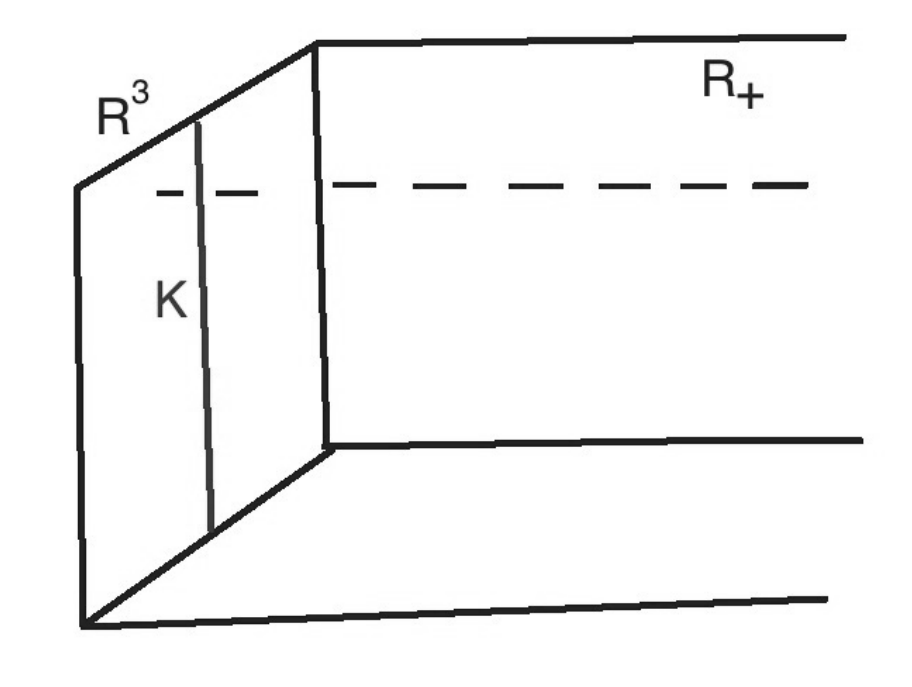
\includegraphics[width=0.46\linewidth]{fig11.png}
  \caption{一个模型情形：纽结由半空间 $\R^4_+$ 边界中的直线 $K=\R$ 表示。
          \quad（原文 Figure~11，第 18 页）}
  \label{fig:11}
\end{figure}

% ===================== 第二讲（续三）：纽结处的模型解 =====================

\subsection{纽结附近的模型解：仿射 Toda 方程}

思路是：在纽结存在的情形下，寻找一个奇异的模型解。
这个解在远离 $K$ 的边界点附近将与 Nahm 极点解一致，但在 $K$ 上的点附近看起来不同。
模型解将依赖于对偶群 $\Gv$ 的一个不可约表示 $R^{\vee}$ 的选取。
于是边界条件定义为：只允许 KW 方程的那些在纽结附近看起来像模型解的解。

% [Tutor Note: 这个“模型解 + 渐近”的边界条件在本节被具体化：
%  远离纽结处 = Nahm 极点（1/y 奇点）；纽结附近 = 新的奇异模型解，
%  以 R^∨ 标号。两个区域之间必须光滑过渡——这正是 [22]（Mazzeo–Witten,
%  “The Nahm Pole Boundary Condition With Knots”）要证明的。
%  注意：R^∨ 的选取不是装饰，它决定了纽结同调的“颜色”（color）；
%  对不同 R^∨ 得到的多项式对应不同表示标号的量子纽结不变量。]

为使这一点有意义，模型解在 $K$ 的任意点附近必须看起来相同，
因此我们假定模型解在沿 $K$ 的平移下不变。于是我们约化到
$\R^2\times\R_+$ 上的方程，此时纽结由 $\R^2$ 中的一点 $p$ 表示（图~\ref{fig:12}）。

\begin{figure}[H]
  \centering
  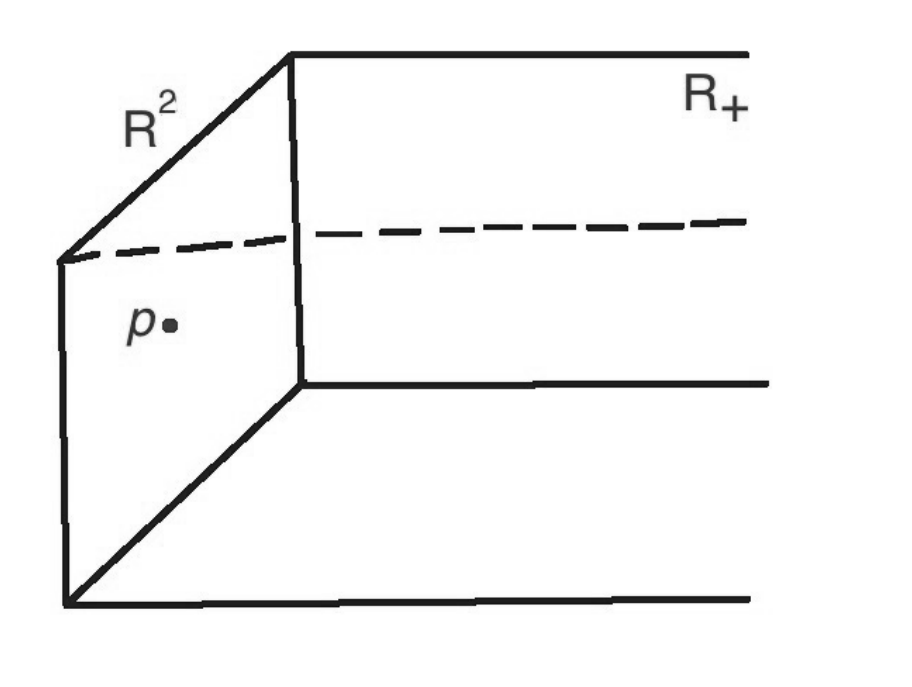
\includegraphics[width=0.46\linewidth]{fig12.png}
  \caption{假定沿图~\ref{fig:11} 中 $K$ 方向平移不变，我们约化到
          $\R^3_+=\R^2\times\R_+$，纽结此时由边界中的点 $p$ 表示。
          \quad（原文 Figure~12，第 19 页）}
  \label{fig:12}
\end{figure}

一旦约化到 3 维（并假定 $A_1$ 与 $\phi_y$ 为零——这一点可由 Weitzenböck 公式给出动机），
KW 方程就变得可以处理了。选取坐标使 $x_1$ 沿纽结 $K$ 方向；
$x_2,x_3$ 参数化边界中 $K$ 的法平面；$y$ 度量到边界的距离。定义三个算子
\begin{equation}\stepcounter{equation}
\begin{aligned}
  \mathcal{D}_1&=\mathcal{D}_2+\mathrm{i}\mathcal{D}_3
    =\frac{\partial}{\partial x_2}+\mathrm{i}\frac{\partial}{\partial x_3}
     +[A_2+\mathrm{i}A_3,\,\cdot\,]\\
  \mathcal{D}_2&=D_y-\mathrm{i}[\phi_1,\,\cdot\,]
    =\frac{\partial}{\partial y}+[A_y-\mathrm{i}\phi_1,\,\cdot\,]\\
  \mathcal{D}_3&=[\phi_2-\mathrm{i}\phi_3,\,\cdot\,],
\end{aligned}
\tag{$\dagger$}\label{eq:Dops}
\end{equation}
以及“矩映射”（moment map）
\begin{equation}\stepcounter{equation}
  \mu=F_{23}-[\phi_2,\phi_3]-D_y\phi_1 .
  \tag{$\ddagger$}\label{eq:mu}
\end{equation}
（原文此处两式均未编号，本文以 $(\dagger)$、$(\ddagger)$ 标记以便引用，原文 p.18。）

% [Tutor Note: 这三行是全文记号最混乱之处，务必看清：
%  (i) 第一行右边的 \mathcal{D}_2、\mathcal{D}_3 是“旧的”协变导数
%      ∂_2+[A_2,·]、∂_3+[A_3,·]；从下一行起 \mathcal{D}_1,\mathcal{D}_2,\mathcal{D}_3
%      被重新定义为三个复算子。同一个符号先旧后新，是原文的记号重载，
%      不是笔误——但极易让读者以为 (†) 是循环定义。
%  (ii) 花体 \mathcal{D} 与普通 D 不同：前者把这些组合算子当成一个整体。
%  (iii) 若把 (1.10) 的符号约定改为 F+φ∧φ，则这里的复结构取 i → −i，
%       \mathcal{D}_2 中 [A_y − iφ_1,·] 的符号随之翻转，需整体一致。
%  (iv) 验证 μ 的来历：μ=0 是 KW 方程中“d_A⋆φ=0 + F_{12},F_{13} 分量”消去后的结果；
%      最直接的办法是把 (1.10) 按 x_2,x_3,y 分量展开并令 ∂_1=0、A_1=φ_y=0。]

在该情形下，KW 方程变为
\begin{equation}\stepcounter{equation}
  0=[\mathcal{D}_i,\mathcal{D}_j],\qquad i,j=1,\dots,3
  \tag{2.13}\label{eq:2.13}
\end{equation}
以及“矩映射”条件
\begin{equation}\stepcounter{equation}
  \mu=0 .
  \tag{2.14}\label{eq:2.14}
\end{equation}

这些方程由 \cite{KW} 引入，被称为\textbf{推广的 Bogomolny 方程}
（extended Bogomolny equations）。它们是规范场论数学中三个被深入研究的方程的混合体。
若丢掉 $\mathcal{D}_1$（即假定场与 $x_2,x_3$ 无关且 $A_2=A_3=0$），就得到 Nahm 方程；
若丢掉 $\mathcal{D}_2$（即假定场与 $y$ 无关且 $A_y=\phi_1=0$），就得到 Hitchin 方程；
若丢掉 $\mathcal{D}_3$（即令 $\phi_2=\phi_3=0$），就得到 Bogomolny 方程。

% [Tutor Note: 这个“三合一”是本文最漂亮的观察之一，值得逐项验证：
%  (i) 丢掉 D_1 后 [D_2,D_3]=0 与 μ=0 合起来给出 dφ_a/dy + ½ε_abc[φ_b,φ_c]=0 —— 即 Nahm 方程；
%  (ii) 丢掉 D_2 后剩下 [D_1,D_3]=0 与 μ=0，即 Hitchin 方程（希格斯丛的自对偶方程）；
%  (iii) 丢掉 D_3 后 [D_1,D_2]=0 与 μ=0 给出 Bogomolny 方程。
%  三者分别对应“沿 y 方向的 ODE”、“沿 x_2,x_3 的二维方程”、“沿三维的方程”。
%  之所以能“混合”，是因为它们都是同一个 4 维方程在不同平移不变性下的约化。]

完整的方程组之所以可处理，原因与它的三个特例各自可处理的原因相同。有两个关键事实：
(a) 方程 $[\mathcal{D}_i,\mathcal{D}_j]=0$ 在 $\Gc$-值规范变换下不变
（$\Gc$ 是 $G$ 的复化）；
(b) 把 $\mu=0$ 与“模去 $G$-值规范变换”合在一起，等价于忘掉 $\mu=0$ 这个条件、
而模去 $\Gc$-值规范变换。这意味着这些解可以用复几何来理解。

% [Tutor Note: 事实 (b) 是 Hitchin 系统/Kähler 商的标准结论：
%  μ=0 且模 G ⇔ 模 G_C（即取复群轨道）。其精确陈述是：
%  复群 G_C 作用在解空间上，每个轨道与 μ^{-1}(0) 的交（模 G）恰为一点。
%  这把“实方程”变成“复几何对象”（全纯丛 + 希格斯场），
%  从而可以用代数几何/复分析的工具。原文说 “equivalent”，
%  严格说是“模空间同构”（Kempf–Ness / Hitchin–Karlhede 型定理），
%  需要稳定性条件；在此处因半单群与紧群的情形而成立。]

可以合理地期望，模型解具有纽结的对称性。因此我们假定，
模型解在边界 $\R^2$ 绕纽结所在点 $p\in\R^2$ 的旋转下不变，
并且在保持 $p$ 固定的 $\R^2\times\R_+$ 缩放变换下不变。
在这些假定下，方程 $[\mathcal{D}_i,\mathcal{D}_j]=\mu=0$ 约化为仿射 Toda 方程，
而后者是可积的。可以找到全部解的封闭形式；并且，满足远离纽结处
Nahm 极点边界条件的解，由对偶群 $\Gv$ 的一个不可约表示 $R^{\vee}$ 分类。
这些解在 $G=SO(3)$、$\Gv=SU(2)$ 的情形下由 \cite{W5branes} 找到，
更一般的情形见 \cite{Mikhaylov}。

% [Tutor Note: “仿射 Toda 方程”在此是 sl(N) 型仿射 Toda 系统（对 G=SU(N)）；
%  R^∨ 的分类作用体现在 Toda 解的“单值性/穿刺点留数”上：
%  不同的不可约表示对应不同的留数（即不同的 Toda 解）。
%  旋转+缩放不变性把 3 维方程降为 1 维（径向）可积系统，这是关键。
%  具体地，su(2) 主嵌入下 Toda 解可用双曲函数显式写出；作者说“closed form”，
%  细节在 [3] §3 与 [25]。这些解正是第二讲边界条件所渐近的模型解。]

% ===================== 第二讲（续四）：椭圆性与结论 =====================

\subsection{椭圆性与 Fredholm 性质}

人们将如何证明：以这些模型方程之一所定义的边界条件，使 KW 方程成为一个
适定（椭圆）的问题？基本上，在关于一致退化椭圆算子的一般性结论之外，
我们需要证明：围绕这些解之一线性化所得的算子 $\sL$ 没有核与余核。
同样只需证明核为零，因为 $\sL^{\dagger}$ 与 $-\sL$ 共轭。

% [Tutor Note: 这里 \sL 再次表示线性化算子（与 p.15 相同），
%  又与第一讲的全纯线丛 \sL 冲突。原文一贯如此，读者按上下文区分即可。]

与无纽结情形完全一样，我们实际上会得到 $\sL$ 核为零的非线性类比：
$\R^3\times\R_+$ 上（纽结如前所述是边界中的一条无限长直线）任何
沿边界并在无穷远处都渐近于模型解的 KW 方程解，实际上与模型解重合。

% [Tutor Note: “非线性消没 ⇒ 线性化核为零”这一步不是形式推导：
%  需要先有解在边界/无穷远处的渐近展开（即 Fredholm 性质与指标），
%  再用隐函数定理把非线性问题线性化。作者在无纽结情形已走过同样的路
%  （p.17），此处说“just as”，是把 [21] 的方法移植到带纽结情形。]

我们想要的消没结果，属于通常可由 Weitzenböck 公式推出的那一类。
但此前考虑过的所有 Weitzenböck 公式，都不适应纽结的存在。
即便那个更精细的、在远离纽结处包含 Nahm 极点奇性的 Weitzenböck 公式
\begin{equation}\stepcounter{equation}
  -\int_M\Tr\bigl(\sV^{2}+\sW^{2}\bigr)=I'+\Delta
  \tag{2.15}\label{eq:2.15}
\end{equation}
也给不出任何有用的信息，因为 $I'$（它是那些在无纽结的 Nahm 极点解中为零的量的平方和）
在纽结存在时是发散的，于是 $I'$ 将为 $+\infty$，从而在纽结存在时 $\Delta$ 将为 $-\infty$。

% [Tutor Note: 式 (2.15) 与 (2.11) 字面相同，是原文的重复编号
%  （作者用它强调“同一个公式在带纽结时失效”）。本译本照录，
%  以便与原文 (2.11)、(2.15) 两处出现一一对应。
%  逻辑与 (2.10) 完全平行：I′ 在 p 点附近发散 ⇒ Δ 发散 ⇒ 公式无用。]

于是我们需要一个新的 Weitzenböck 公式。我们模仿此前的做法：
找一族量 $X_i$，其为零恰好刻画模型解。
（一些明显的 $X_i$ 是 $[\mathcal{D}_i,\mathcal{D}_j]$ 的实部与虚部，以及 $\mu$；
另一些则是像 $[\phi_i,\phi_y]$ 这样因模型解有 $A_1=\phi_y=0$ 而为零的量。）
于是若
\begin{equation}\stepcounter{equation}
  I''=-\sum_{i}\int_{\R^3\times\R_+}\Tr X_i^{2},
  \tag{2.16}\label{eq:2.16}
\end{equation}
我们就得期望存在恒等式
\begin{equation}\stepcounter{equation}
  -\int_{\R^3\times\R_+}\Tr\bigl(\sV\wedge\star\sV+\sW\wedge\star\sW\bigr)
  =I''+\widehat{\Delta},
  \tag{2.17}\label{eq:2.17}
\end{equation}
其中 $\widehat{\Delta}$ 是一个新的边界项。结果表明，这样的恒等式确实存在。

% [Tutor Note: (2.16)--(2.17) 是全文最后的技术核心，也是 [22] 的主要工作。
%  与 (2.11) 的区别在于：I″ 的平方和是针对“带纽结的模型解”选取的 X_i，
%  因此在 p 点附近不再发散（模型解本身的奇性被吸收进 X_i 的构造）。
%  这一步相当于在 Mazzeo 的 edge calculus 中选取合适的“模型算子”与
%  “指标配对”；作者说 “It turns out”，是因为完整验证在 [22] 中。]

我们仍需证明：在解满足 KW 方程、且在纽结附近渐近于模型解的情形下，
$\widehat{\Delta}=0$。为此，需要知道 KW 方程的解在边界附近与无穷远处的渐近行为。
我们已经知道一般边界点处的行为（这在证明无纽结时 Nahm 极点边界条件的适定性时用过）。
为求纽结附近以及无穷远处的行为，现在需要在二维半球面 $S^2_+$ 上解方程的角向部分（图~\ref{fig:13}）。

\begin{figure}[H]
  \centering
  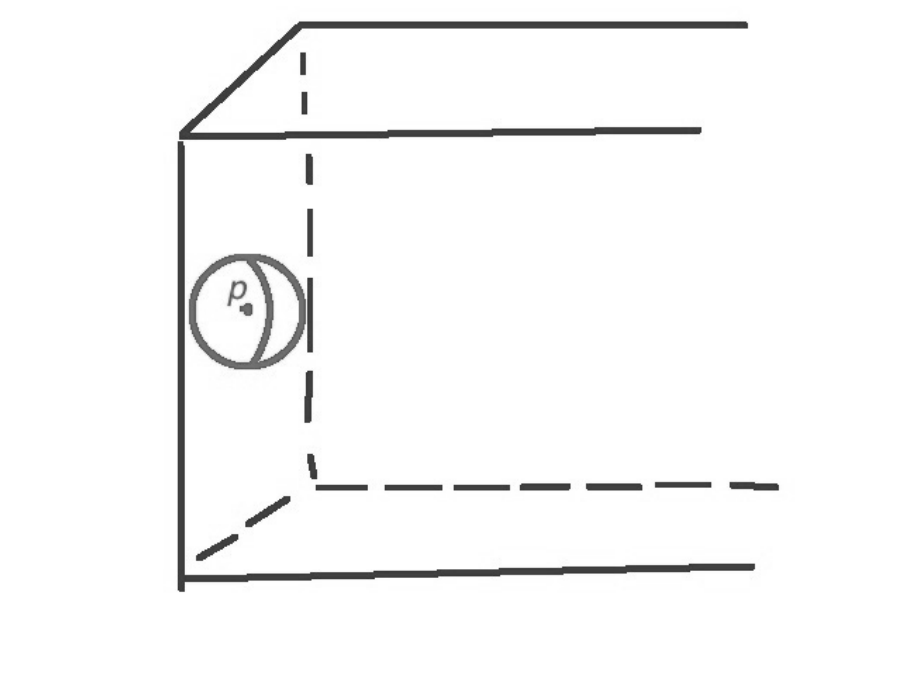
\includegraphics[width=0.46\linewidth]{fig13.png}
  \caption{为在纽结存在时证明消没定理，须研究边界上奇点附近的角向算子。
          该角向算子定义在图中所示的半球面上。\quad（原文 Figure~13，第 21 页）}
  \label{fig:13}
\end{figure}

再次地，角向算子的本征值是有利的，因此无论在 $p$ 附近还是在无穷远处，
$\widehat{\Delta}$ 都没有贡献。这一事实连同相关的 Weitzenböck 公式表明：
$\R^3\times\R_+$ 上、在边界与无穷远处都渐近于带纽结模型解的 KW 方程解，
实际上与该模型解重合。

% [Tutor Note: “角向算子”在此是 S²₊（半球面）上的算子，因为约化到
%  R²×R₊ 后，绕 p 的旋转群是 SO(2)⊂SO(3)，其角向部分落在 S²₊ 上；
%  与无纽结情形（S³₊）相比降了一维。作者两次说“本征值有利”，
%  背后的计算是 [22] 的核心，且涉及非平凡的特殊函数（超几何型）。
%  若要做数值/符号验证，这是最值得投入的地方。]

同一论证的线性化版本表明 $\sL$ 的核为零，而这正是我们为证明椭圆性所需要知道的。

这就是证明 $\sL$ 在任意嵌入于任意三维流形 $W$ 中的纽结 $K$ 存在时
仍为 Fredholm 算子的主要一步。要证明这在弯曲纽结的一般情形下给出
非线性 KW 方程的椭圆边界条件，还有一些细节需要补充（见 \cite{MWknots}）。

% [Tutor Note: 最后一句话点明了本文的未完成之处：
%  (i) 弯曲纽结（K 不直）时，模型解需要在法向标架上“粘合”，
%      涉及非平凡的和乐（holonomy）与过渡函数；
%  (ii) 5 维情形（范畴化）尚未逐字写出；
%  (iii) 紧致性（(2.2) 的有限项）仍未证明。
%  这三点正是 [22] 与后续工作的主题。引用本文时应把结论限定为
%  “在模型情形（直纽结、4 维）已证明，一般情形待补”。]

% ===================== 附录 A：一些物理背景 =====================
\appendix
\section{一些物理背景（Some Physics Background）}
\label{sec:appendix}

\begin{keypoints}
  \item \textbf{物理图像}：单分次 Khovanov 同调对应六维 $(0,2)$ 超共形理论
        经过“拓扑—全纯扭曲”并沿 $S^1$ 紧化后的低能有效理论（5 维最大超对称
        规范理论）；而双分次版本对应把紧化曲面从 $\CC^{*}=\R\times S^1$
        换成 $\CC$（即保留一个 $S^1$ 作用，对应第二分次）。
  \item \textbf{数学工具}：$(0,2)$ 理论、R 对称性 $Spin(5)$、类 $S$ 理论、
        半 BPS 面算子、't Hooft 型面算子、Langlands–GNO 对偶。
  \item \textbf{核心结论}：面算子只能沿 $p\times C$ 或 $\Sigma\times q$ 放置，
        原因是 $C$ 的全纯子流形只有 $C$ 本身与点；把 $S^1$ 收缩掉就得到
        4 维/5 维规范理论中的 $S\subset W_3$ 条件——这就从物理上解释了
        第一讲“为什么 1-流形必须落在三维切片里才能有打结性”。
\end{keypoints}

在本附录中，我将简要描述第一讲中处理单分次 Khovanov 同调时的一些物理背景。
关于弦/M 理论的语境，以及 \cite{W5branes} 中处理双分次 Khovanov 同调的框架，
这里只给出一个粗略轮廓。我的主要目的是解释：对单分次理论而言，
不同之处究竟在哪里。

% [Tutor Note: 附录的定位要看清：它不是在证明数学定理，而是在解释
%  “第一讲的那些方程从哪来”。作者明说 “bare outline”，
%  因此任何细节都需回溯 [3]（Fivebranes and knots, 1101.3216）。
%  阅读时把附录与正文对照：正文的 KW/HW 方程 ←→ 附录的 (0,2) 理论扭曲。]

\subsection{六维 (0,2) 理论与拓扑—全纯扭曲}

出发点是如下六维超共形场论的存在性：它具有 $(0,2)$ 超对称，
与任意单边（simply-laced）Lie 群 $G$ 相联系——更确切地说，与其 Dynkin 图相联系。
该理论具有 $Spin(5)$ 的 R 对称性群。利用子群 $F=Spin(2)\subset Spin(5)$，
可以对该理论作拓扑扭曲，使其能紧化在 Riemann 曲面 $C$ 上，
给出一个具有 $\mathcal{N}=2$ 超对称的四维理论。
这些就是类 $S$（class $S$）理论，见 \cite{GaiottoN2} 的研究。
它们具有 R 对称性群
$\widehat{F}=\bigl(Spin(3)\times Spin(2)\bigr)/\ZZ_2\cong U(2)$
（即 $Spin(5)$ 中与 $F$ 对易的子群）。
利用 $Spin(3)$ 因子，类 $S$ 理论可以被拓扑扭曲并紧化在四维流形 $M$ 上，
同时保持一个超荷 $Q$。这给出 $M\times C$ 上的一个理论，
它沿 $M$ 是拓扑的、沿 $C$ 是全纯的。
（沿 $C$ 的全纯性意味着，例如：$Q$ 作用在 $M\times C$ 上局部算子所得的上同调，
作为 $C$ 上的对象是全纯变化的。）
$M\times C$ 上这个“拓扑—全纯”理论仍具有 $F=Spin(2)$ 对称性，
因为 $F$ 与用于扭曲的群 $\widehat{F}$ 对易。

% [Tutor Note: 这一段的信息密度极高，逐句对应如下：
%  (0,2) 六维 SCFT ←→ 单边 Lie 群的 Dynkin 图（ADE 分类）；
%  Spin(5)_R 的 5 维表示分解为 Spin(2)×Spin(3)：F=Spin(2) 用于拓扑扭曲
%  （把 F 的自旋联络代入，使 Q 成为标量），剩下的 Spin(3) 用于
%  在 M 上的拓扑扭曲。两重扭曲叠加即 “topological-holomorphic”。
%  “class S” 指 Gaiotto 的 N=2 理论族；其 R 对称性 U(2) 来自 Spin(5) 的
%  中心化子。若读者只关心结果，可记住：这一整套 twisting 的净效果
%  就是让 6 维理论在 M×C 上变成 4 维 KW 方程 + 沿 C 的全纯依赖。]

\subsection{面算子、紧化与 HW 方程}

底层的六维 $(0,2)$ 模型允许半 BPS 面算子（surface operators），
它们可以支撑在六维中的任意二维流形 $U$ 上。
然而，当该理论如上一段所述被表述在 $M\times C$ 上时，
若我们希望保持拓扑—全纯理论的超荷 $Q$，则 $U$ 的可能选取相当受限。
$U$ 必须具有形式 $p\times C$（$p$ 是 $M$ 中的点），或
$\Sigma\times q$（$\Sigma\subset M$ 是二维流形，$q$ 是 $C$ 中的点）。
其原因本质上是：$C$ 的任何（完备、连通的）全纯子流形，
或者是 $C$ 本身，或者是一个点 $q\in C$。
为构造 Khovanov 同调，我们取 $U=\Sigma\times q$。

% [Tutor Note: “$C$ 的全纯子流形只有 $C$ 与点”这一句在本附录中是关键：
%  $C$ 是复曲线，故其全纯子流形只能是 0 维或 1 维（连通、完备）。
%  这条几何事实决定了面算子不能“斜着”放置——从而解释了第一讲中
%  “S 必须落在 3 维切片里”的物理起源。作者在第一讲说 “see the appendix”，
%  指的就是这里。注意 $p\times C$ 型面算子对偶于 4 维中的“点算子”，
%  而 $\Sigma\times q$ 型对偶于 4 维中的“面算子”。]

\subsection{单分次与双分次的区别}

为得到单分次 Khovanov 同调，我们取 $M$ 为 $\R^4$、$C$ 为圆柱
$\R\times S^1$。六维流形 $M\times C$ 于是就是 $\R^4\times\R\times S^1$。
超荷 $Q$ 在 $\R^4$ 的旋转下不变（与 $Spin(3)\subset\widehat{F}$ 的适当元素联合），
但在 $\R^4\times\R$ 的更一般旋转下不变。
现在利用如下事实：$(0,2)$ 模型在任意五维流形 $M'$ 上的 $M'\times S^1$ 形式中，
当 $M'$ 的半径远大于 $S^1$ 的半径时，在 $M'$ 上的长距离下约化为
以 $G$ 为规范群的极大超对称规范理论。在上述拓扑—全纯理论的语境中，
这一约化无需取任何大距离极限即成立。所得的 $M'=\R^4\times\R$ 上的
超对称规范理论是红外自由的（与六维中底层的 $(0,2)$ 模型形成鲜明对比），
因此可以用经典方法分析。特别地，$Q$-不变性的条件变成 HW 方程——
第一讲中已提到。它们是关于一对场的方程：规范场 $A$，以及 $\R^4\times\R$ 上的场 $B$；
$B$ 是 $\R^4$ 上自对偶 2-形式丛拉回到 $\R^4\times\R$ 后的、取伴随值的截面。

% [Tutor Note: 这里出现本文与 [15]/[3] 的接口：“$B$ 是自对偶 2-形式的伴随值截面”。
%  在 [3] 的记号里，HW 方程是五维的、含 A 与 B 两个场（B 为自对偶 2-形式）；
%  本文正文用的是 4 维 KW 方程的 (A,φ) 表述。二者的对应是：
%  沿 S¹ 约化后，φ 的 u-分量与 B 的某分量配对，B 的其余分量给出 4 维方程中的
%  φ（1-形式）与辅助场。作者在此只说 “mentioned in Lecture One”，
%  未给对照表；要做严格对应，须查 [3] §2 或 [15] §3.3。]

六维中支撑在 $\Sigma\times q$ 上的面算子，在规范理论描述中约化为
支撑在 $\Sigma\times q'$ 上的 't Hooft 型面算子，其中 $q\in\R\times S^1$
投影到 $q'\in\R$。含有该面算子时 HW 方程的解，应当沿 $\Sigma\times q'$
具有奇点。这个余维 3 的奇点应当以 Bogomolny 方程的标准余维 3 奇点为模型，
并适当地嵌入以 $G$ 为规范群的 HW 方程中。

% [Tutor Note: “'t Hooft 型面算子”即 't Hooft 在 1978 年引入的那种
%  在面上去除规范场奇异性的算子（'t Hooft loop 的二维推广），
%  其定义正是“要求场的奇点沿面具有规定形式”——与本文正文的
%  “边界条件 = 指定奇异模型解”是同一思想在 4 维/5 维中的体现。
%  作者在正文引用 [14]（'t Hooft）时，指的就是这个构造。]

为范畴化与单边紧 Lie 群 $\Gv$ 的表示 $R^{\vee}$ 相联系的量子纽结不变量，
人们研究以 $G$ 为规范群（$G$ 是 $\Gv$ 的 Langlands–GNO 对偶；
特别地，若 $G$ 单边，则 $G$ 与 $\Gv$ 具有相同的 Lie 代数）、
并沿 $\Sigma\times q'$ 具有适当奇点的 HW 方程。
如第一讲所述，适当的奇点是通过同态 $\rho:\ug\to\mathfrak{t}\subset\Lie$
把奇异 $U(1)$ 解嵌入 $G$ 而得到的，其中 $\rho$ 与 $R^{\vee}$ 对偶。

% [Tutor Note: 若 G^∨ 不是单边群，则需要 [3] §5.5 描述的修正（脚注 5），
%  因为此时 G 与 G^∨ 的 Lie 代数不同，嵌入需经过“非单边”的推广。
%  这是本文与 [3] 的一个技术接口，正文未展开。]

$\R^4\times\R$ 上的 HW 方程，与二维流形 $V\subset\R^4\times\R$ 上
熟悉的余维 3 奇点相容，当且仅当 $V$ 具有形式 $\Sigma\times q'$，
其中 $\Sigma\subset\R^4$、$q'\in\R$。
这一陈述通过检查 HW 方程即可容易地验证。
我们这里从 $(0,2)$ 模型出发给出的解释，有助于说明“为什么”它成立。

% [Tutor Note: 原文此处写作 “V ⊂ R⁴ × q′ ⊂ R⁴ × R”，从上下文看应为
%  “V ⊂ Σ × q′”（或 M × q′），因为上一句刚定义了 V = Σ × q′、Σ ⊂ R⁴。
%  这很可能是作者笔误或 dvips 转换中的记号丢失（R⁴ 与 Σ 的字形不同，
%  但排版上易混）。本译本照录原文，并在此标注；引用时建议按 Σ × q′ 理解。]
把 $V$ 限制为 $V\subset\R^4\times q'\subset\R^4\times\R$，
对于从这一构造中得到纽结理论而言是完全本质的：
若 $V$ 可以在五维中自由移动，相关的拓扑就会消失。
例如，Khovanov 同调出现在“时间”无关的情形
$\Sigma=\R_t\times K\subset\R_t\times\R^3=\R^4$，
其中 $K$ 是 $\R^3$ 中的纽结，$\R^4=\R_t\times\R^3$ 的第一个因子由“时间”参数化。
若 $V$ 可以在 $\R^4\times\R$ 中自由变化，则 $K$ 就可以在 $\R^3\times\R$
（即 $\R^4\times\R=\R_t\times\R^3\times\R$ 中后两个因子的乘积）中自由变化，
从而可以被平凡地解结。第一讲中也表达了大致相同的要点。
更一般的 $V$（不具有时间无关形式 $\R_t\times K$）被用来定义
Khovanov 同调的“态射”。

% [Tutor Note: 这段是把“为什么 1-流形在 4 维中不打结”翻译成物理语言：
%  打结性来自 K 在 3 维切片中的嵌入；若允许 V 在 5 维中自由移动，
%  则 K 可以在 4 维中任意变形，任何纽结都平凡。这与第一讲
%  “singled-graded becomes trivial after decategorification” 是同一件事的
%  两种说法。注意原文 “A more general V ... is used to define the morphisms”
%  指的是 Khovanov 同调的 cobordism 映射（V 为带边的 2-维协边）。]

我们所描述的对应于 Khovanov 同调的单分次版本
（只有上同调分次，没有“$q$”-分次）。
单分次来自整个构造中保持的对称群 $F\cong Spin(2)$。
为得到双分次 Khovanov 同调，人们取 $C$ 不是 $\CC^{*}=\R\times S^1$ 而是 $\CC$。
做法是在 $\CC^{*}$ 上添加一个“在无穷远处”的点 $q_0$。
$\CC$ 具有一个 $S^1$ 作用，固定点 $q_0$。
在底层的 $(0,2)$ 模型中，人们考虑支撑在 $U=\Sigma\times q_0$ 上的面算子。
把 $M\times C$ 沿 $S^1$ 的轨道约化，现在给出 $M\times\R_+$ 上规范理论的描述
（其中 $\R_+$ 是半直线，即商 $C/S^1$）。
$S^1$ 作用给出所需的第二分次。
这一构造的双分次版本是 \cite{W5branes} 的主要论题，此处不再重复其细节。

% [Tutor Note: 最后一段解释了“为什么双分次需要 C = C 而不是 C*”：
%  C* = R×S¹ 上 S¹ 作用无固定点，约化后只剩 R（即 y 方向），
%  没有额外的 U(1) 对称性；而 C 上 S¹ 作用有一个固定点 q₀，
%  剩余作用在 C/S¹ = R₊ 的“内部”仍有一个 U(1)（绕 q₀ 的旋转），
%  这个 U(1) 正是 q-分次的来源。这是全文最精妙的几何—物理对应之一，
%  也是 [3] 与本文的分水岭：本文只处理单分次（C*），
%  [3] 处理双分次（C）。]

\subsection*{致谢}
本研究部分受 NSF 基金 PHY-1314311 资助。感谢 M. Abouzaid、C. Manolescu
与 R. Mazzeo 的有益讨论。

% ===================== 参考文献 =====================
\newpage
\begin{thebibliography}{99}
\small

\bibitem{GVS} S. Gukov, A. S. Schwarz, and C. Vafa,
  ``Khovanov-Rozansky Homology And Topological Strings,''
  Lett. Math. Phys. \textbf{74} (2005) 53--74, hep-th/0412243.

\bibitem{OV} H. Ooguri and C. Vafa, ``Knot Invariants And Topological Strings,''
  Nucl. Phys. \textbf{B577} (2000) 419, hep-th/9912123.

\bibitem{W5branes} E. Witten, ``Fivebranes And Knots,''
  Quantum Topology \textbf{3} (2012) 1--137, arXiv:1101.3216.

\bibitem{WKhovanovGauge} E. Witten, ``Khovanov Homology and Gauge Theory,''
  in R. Kirby, V. Krushkal, and Z. Wang, eds.,
  \emph{Proceedings Of The FreedmanFest} (Mathematical Sciences Publishers, 2012) 291--308,
  arXiv:1108.3103.

\bibitem{WtwoLectures} E. Witten, ``Two Lectures On The Jones Polynomial And Khovanov Homology,''
  arXiv:1401.6996.

\bibitem{SS} P. Seidel and I. Smith, ``A Link Invariant From The Symplectic Geometry
  of Nilpotent Slices,'' Duke Math. J. \textbf{134} (2006) 453--514.

\bibitem{Manolescu} C. Manolescu, ``Nilpotent Slices, Hilbert Schemes, and the Jones Polynomial,''
  Duke Math. J. \textbf{132} (2006) 311--369.

\bibitem{AS} M. Abouzaid and I. Smith, ``Khovanov Homology From Floer Cohomology,''
  arXiv:1504.01230.

\bibitem{Jones} V. F. R. Jones, ``A Polynomial Invariant For Knots Via Von Neumann Algebra,''
  Bull. Am. Math. Soc. \textbf{12} (1985) 103--111.

\bibitem{Atiyah} M. F. Atiyah, ``Floer Homology,'' Progr. Math. \textbf{133} (1995) 105.

\bibitem{GW} D. Gaiotto and E. Witten, ``Knot Invariants From Four-Dimensional Gauge Theory,''
  Adv. Theor. Math. Phys. \textbf{16} (2012) 935, arXiv:1106.4789.

\bibitem{Kamnitzer} J. Kamnitzer, ``The Beilinson-Drinfeld Grassmannian and Symplectic Knot Homology,''
  in D. A. Ellwood (ed.), \emph{Grassmannians, Moduli Spaces, and Vector Bundles}
  (Clay Math Institute, Cambridge MA and American Mathematical Society, Providence RI, 2011) 81--94.

\bibitem{CK} S. Cautis and J. Kamnitzer, ``Knot Homology Via Derived Categories Of Coherent Sheaves,
  I. The $\mathfrak{sl}(2)$ Case,'' Duke Math. J. \textbf{142} (2008) 511--588.

\bibitem{tHooft} G. 't Hooft, ``On The Phase Transition Towards Permanent Quark Confinement,''
  Nucl. Phys. \textbf{B138} (1978) 1--25.

\bibitem{KW} A. Kapustin and E. Witten, ``Electric-Magnetic Duality And The Geometric Langlands Program,''
  Commun. Numb. Th. Physics \textbf{1} (2007) 1--236.

\bibitem{Bigelow} S. Bigelow, ``A Homological Definition Of The Jones Polynomial,''
  Geometry and Topology Monographs, Volume 4: \emph{Invariants of Knots and 3-Manifolds}
  (Kyoto, 2001), pp. 29--41.

\bibitem{Lawrence} R. Lawrence, ``A Functorial Approach to the One-Variable Jones Polynomial,''
  J. Diff. Geom. \textbf{37} (1993) 689--710.

\bibitem{GalakhovMoore} D. Galakhov and G. W. Moore, ``Comments On The Two-Dimensional
  Landau-Ginzburg Approach,'' arXiv:1607.04222.

\bibitem{Haydys} A. Haydys, ``Fukaya-Seidel Category And Gauge Theory,''
  J. Symp. Geom. \textbf{13} (2015) 151--207, arXiv:1010.2353.

\bibitem{GPV} S. Gukov, P. Putrov, and C. Vafa, ``Fivebranes and 3-manifold Homology,''
  arXiv:1602.05302.

\bibitem{MW} R. Mazzeo and E. Witten, ``The Nahm Pole Boundary Condition,''
  in \emph{The Influence Of Solomon Lefschetz in Geometry and Topology},
  ed. L. Katzarkov et al. (American Mathematical Society, 2014), arXiv:1311.3167.

\bibitem{MWknots} R. Mazzeo and E. Witten, ``The Nahm Pole Boundary Condition With Knots,''
  to appear.

\bibitem{Nahm} W. Nahm, ``All Selfdual Multimonopoles for Arbitrary Gauge Groups''
  (NATO ASI, 1983).

\bibitem{Corlette} K. Corlette, ``Flat $G$-Bundles With Canonical Metric,''
  J. Diff. Geom. \textbf{28} (1988) 361--382.

\bibitem{Mikhaylov} V. Mikhaylov, ``On The Solutions Of Generalized Bogomolny Equations,''
  JHEP \textbf{05} (2012) 112, arXiv:1202.4848.

\bibitem{GaiottoN2} D. Gaiotto, ``$\mathcal{N}=2$ Dualities,'' JHEP \textbf{1208} (2012) 034,
  arXiv:0904.2715.

\end{thebibliography}

\end{document}

